\documentclass[10pt]{beamer}

\usepackage[utf8]{inputenc}
\usepackage[swedish, english]{babel}
\usepackage{epstopdf}
\epstopdfsetup{update} % only regenerate pdf files when eps file is newer
\usepackage[squaren]{SIunits}
\usepackage{subfig}
\captionsetup[subfigure]{labelformat=empty}
\usepackage{array}
\newcolumntype{P}[1]{>{\raggedright\arraybackslash}p{#1}}

\usetheme[progressbar=frametitle]{metropolis}

\usepackage{booktabs}
\usepackage[scale=2]{ccicons}

\usepackage{pgfplots}
\usepgfplotslibrary{dateplot}

\usepackage{xspace}
\newcommand{\themename}{\textbf{\textsc{metropolis}}\xspace}

\usepackage{media9}


%\setbeamertemplate{frame footer}{Niklas Ericson - Linköping University}
\setbeamercolor{progress bar}{ fg = CERNBlue , bg = CERNBlue!30 }
\setbeamercolor{alerted text}{ fg = CERNBlue , bg = CERNBlue!30 }
\setbeamercolor{background canvas}{ fg = white , bg = white }

\title{Presentation of Master's Thesis}
\subtitle{Investigation of Control Approaches for a High Precision, \\ Piezo-actuated Rotational Stage}
\date{\today}
\author{Niklas Ericson}
\institute{Linköping University | European Organization for Nuclear Research}
\titlegraphic{\hfill\includegraphics[height=1cm, trim=0cm 0.65cm 0cm 0cm, clip=true]{../fig/LiU_primary_black}
              \hspace{0.2cm}\includegraphics[height=1.2cm]{../fig/CERNLogoBadge}}

\begin{document}

\maketitle

\begin{frame}{Table of contents}
  \setbeamertemplate{section in toc}[sections numbered]
  \tableofcontents[hideallsubsections]
\end{frame}

\section{Introduction}

\begin{frame}[fragile]{CERN}
  The Large Hadron Collider (LHC) at CERN.
\center
\includemedia[
  width=0.8\linewidth,height=0.5\linewidth,
  activate=pageopen,
  flashvars={
    modestbranding=1 % no YT logo in control bar
   &autohide=1       % controlbar autohide
   &autoplay=1
   &cc_load_policy=1
   &showinfo=0       % no title and other info before start
   &start=32
   &end=55
  }
]{}{http://www.youtube.com/v/h2-ocLjUhTU?rel=0}   % Flash file
\\
Source: \cite{youtube}.
\end{frame}

\begin{frame}[fragile]{Collimation}
  Collimation system used in the LHC.
\center
\includemedia[
  width=0.8\linewidth,height=0.5\linewidth,
  activate=pageopen,
  flashvars={
    modestbranding=1 % no YT logo in control bar
   &autohide=1       % controlbar autohide
   &autoplay=1
   &cc_load_policy=1
   &showinfo=0       % no title and other info before start
   &start=76
   &end=121
  }
]{}{http://www.youtube.com/v/h2-ocLjUhTU?rel=0}   % Flash file
\\
Source: \cite{youtube}.
\end{frame}

\begin{frame}[fragile]{Crystal Collimation}
  The UA9 collaboration at CERN investigates how bent crystals can be used to extract halo particles.

  \begin{figure}[h!]
    \centering %crop: left bottom right top
    \includegraphics[width=1\textwidth, trim= 2cm 15.5cm 1cm 10cm, clip=true]{../fig/matlab/collimation}
    \caption{\label{fig:collimation}Illustration of the crystal collimation principle.}
  \end{figure}

  Implies in a more efficient cleaning, a less complex system and a reduction of the machine impedance.
\end{frame}

\begin{frame}[fragile]{Purpose and Goal}
  The \textbf{ higher the energy} of the particle the \textbf{lower the angular acceptance} for channeling.
  \begin{itemize}
    \item have a total range of \unit{20}{\milli\rad}
    \item be able to track reference trajectories at ramp rates of \unit{100}{\micro\radianpersecond}
    \item reject external disturbances to maintain a maximum tracking error of $\pm$\unit{1}{\micro\rad} even when the linear axis is moving
  \end{itemize}
\end{frame}

\begin{frame}[fragile]{Challenges}
  \begin{itemize}
    \item Nonlinear effect such as hysteresis and creep
    \item Highly resonant structure
    \item The linear movement adds additional perturbation
    \item System changes due to rotational and linear position, moving center of rotation.
  \end{itemize}
\end{frame}

\begin{frame}[fragile]{Method}
  \begin{itemize}
    \item Literature study
    \item Further investigation of selected control approaches
    \item Benchmarking tests of selected control approaches in simulations
    \item Implementation of the most promising approach
    \item Proposal of controller
  \end{itemize}
\end{frame}

\section{System Overview}

\begin{frame}[fragile]{Crystal Collimator}
  \begin{figure}[h]
    \centering %crop: left bottom right top
    \subfloat[][\label{fig:collimator-side}Side view]{
    \includegraphics[width=0.4\textwidth, trim=2cm 11cm 2cm 5cm, clip=true]{../fig/collimator-side}}
    \qquad
    \subfloat[][\label{fig:collimator-top}Top view]{
    \includegraphics[width=0.4\textwidth, trim=0cm 0cm 0cm 0cm, clip=true]{../fig/collimator-top}}
    \caption{\label{fig:collimator} The new collimator from the side (a) and the top (b).}
  \end{figure}
\end{frame}

\begin{frame}[fragile]{Crystal Collimator}
  \begin{figure}[h!]
    \centering %crop: left bottom right top
    \subfloat[][\label{fig:collimator-through} Giving access]{
    \includegraphics[width=0.4\textwidth, trim=3cm 12.8cm 2cm 5cm, clip=true]{../fig/collimator-through}}
    \qquad
    \subfloat[][\label{fig:collimator-mirror} Insertion of crystal]{
    \includegraphics[width=0.4\textwidth, trim=0cm 0cm 0cm 0cm, clip=true]{../fig/collimator-mirror}}
    \caption{\label{fig:collimator-t} The new collimator with the beam pipe piece half-way out (a) and the crystal inserted into the beam pipe (b).}
  \end{figure}
\end{frame}

\begin{frame}{Rotational Stage}
  \begin{itemize}
    \item Monolithic structure to avoid sliding parts
    \item Piezoelectric stack actuator
    \item Displacement: 0 to \unit{30}{\micro\meter} $\implies$ 0 to 20 mrad
    \item Nonlinear effects
  \end{itemize}

  \begin{figure}[h!]
    \centering %crop: left bottom right top
    \subfloat[][]{
    \includegraphics[width=0.45\textwidth]{../fig/rotational-stage.jpg}}
    \qquad
    \subfloat[][]{
    \includegraphics[width=0.45\textwidth]{../fig/rotational-stage-interferometer.jpg}}
  \end{figure}
\end{frame}

\begin{frame}{Modeling}
  \begin{itemize}
    \item \alert{Hysteresis effect} - Modeled by a Maxwell slip model
    \item \alert{Creep effect} - Efficiently eliminated in closed loop
    \item \alert{Rotational stage} - modeled as a Hammerstein structure
  \end{itemize}

  \begin{figure}[h]
    \centering %crop: left bottom right top
    \includegraphics[width=0.55\textwidth, trim=8cm 8cm 7.73cm 8cm, clip=true]{../fig/matlab/hammerstein}
    %\caption{\label{fig:hammerstein}Block diagram of a Hammerstein structure, consisting of two blocks in series, modeling the static hysteresis and the linear dynamics, respectively.}
  \end{figure}
  \vspace{-1cm}

  \begin{figure}[h]
    \centering %crop: left bottom right top
    \subfloat[][]{
    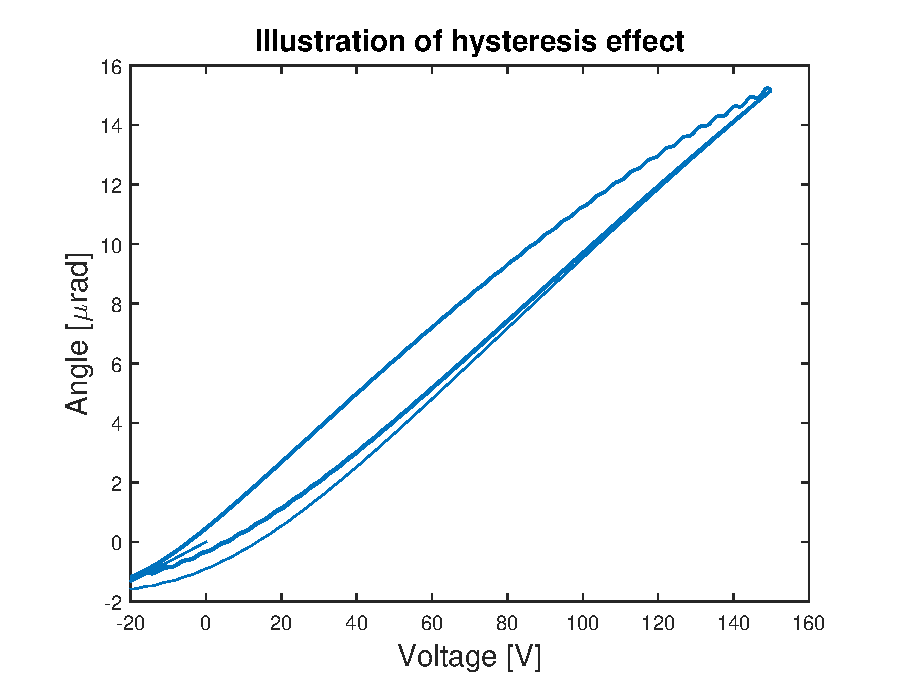
\includegraphics[width=0.27\textwidth]{../fig/matlab/hysteresis.eps}}
    \qquad
    \subfloat[][]{
    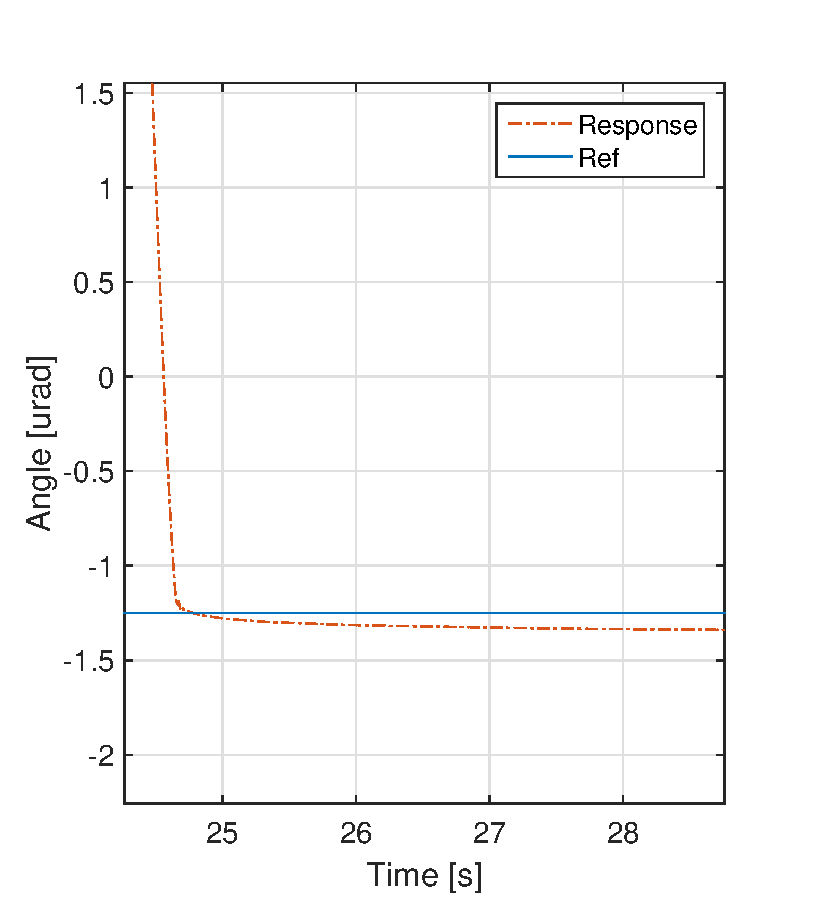
\includegraphics[width=0.27\textwidth]{../fig/matlab/creep.eps}}
    \qquad
    \subfloat[][]{
    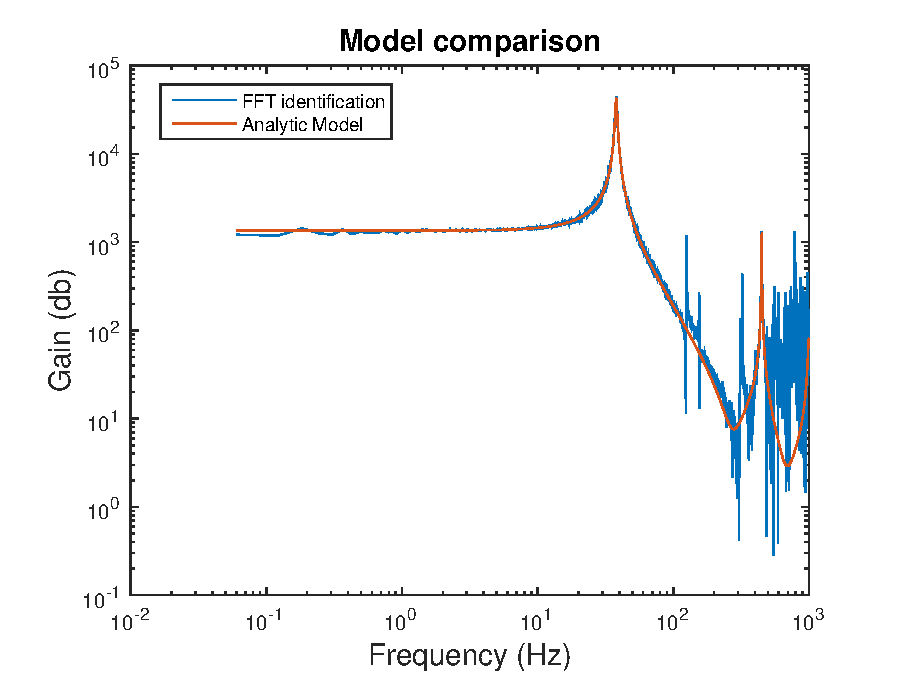
\includegraphics[width=0.27\textwidth]{../fig/matlab/model.eps}}
  \end{figure}
\end{frame}

\begin{frame}{Linear System Identification}
  \begin{figure}[h!]
    \centering
    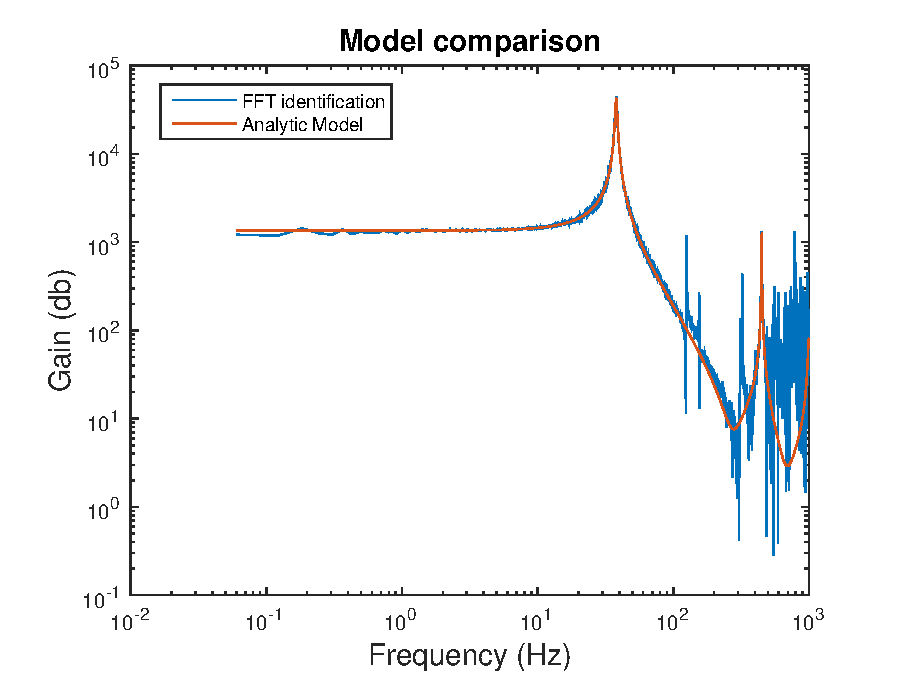
\includegraphics[width=0.7\textwidth]{../fig/matlab/model.eps}
    \caption{\label{fig:model} Model fit of the system model with 5 zeros and 6 poles to the FFT of the acquired data.}
  \end{figure}
\end{frame}

\begin{frame}{Linear System Identification}
  \begin{figure}[h]
    \centering %crop: left bottom right top
    \subfloat[][\label{fig:different_angles}Different rotational head positions]{
    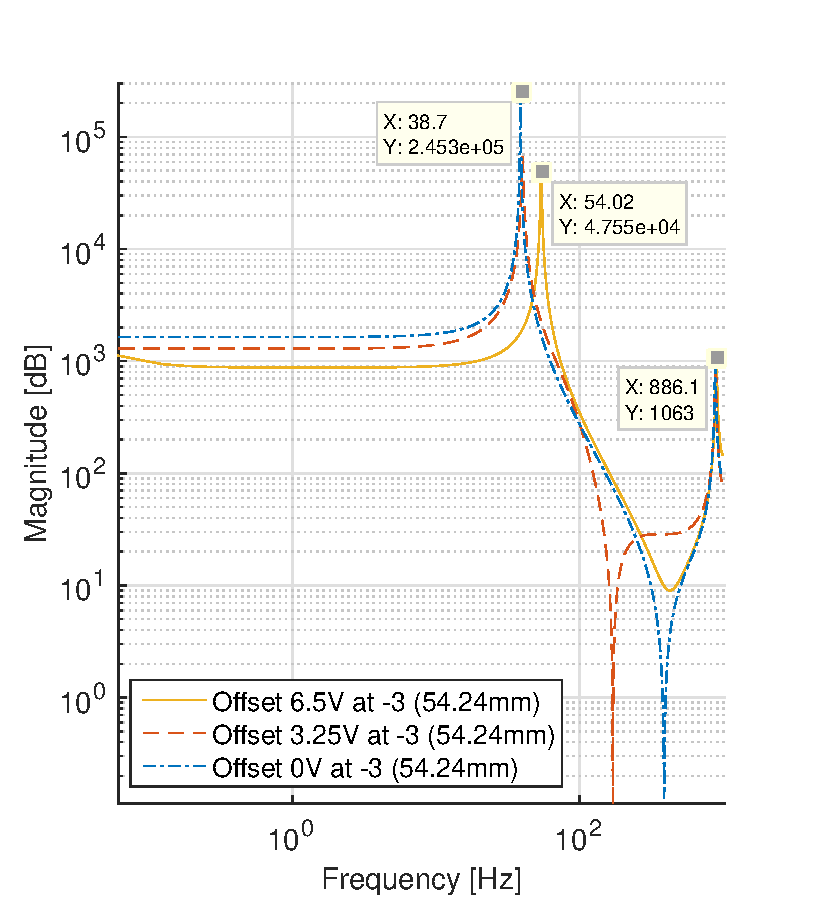
\includegraphics[width=0.4\textwidth, trim=0cm 0cm 0.8cm 1cm, clip=true]{../fig/matlab/modelcomparison_diffvolt2.eps}}
    \qquad
    \subfloat[][\label{fig:different_lin_pos}Different linear axis positions]{
    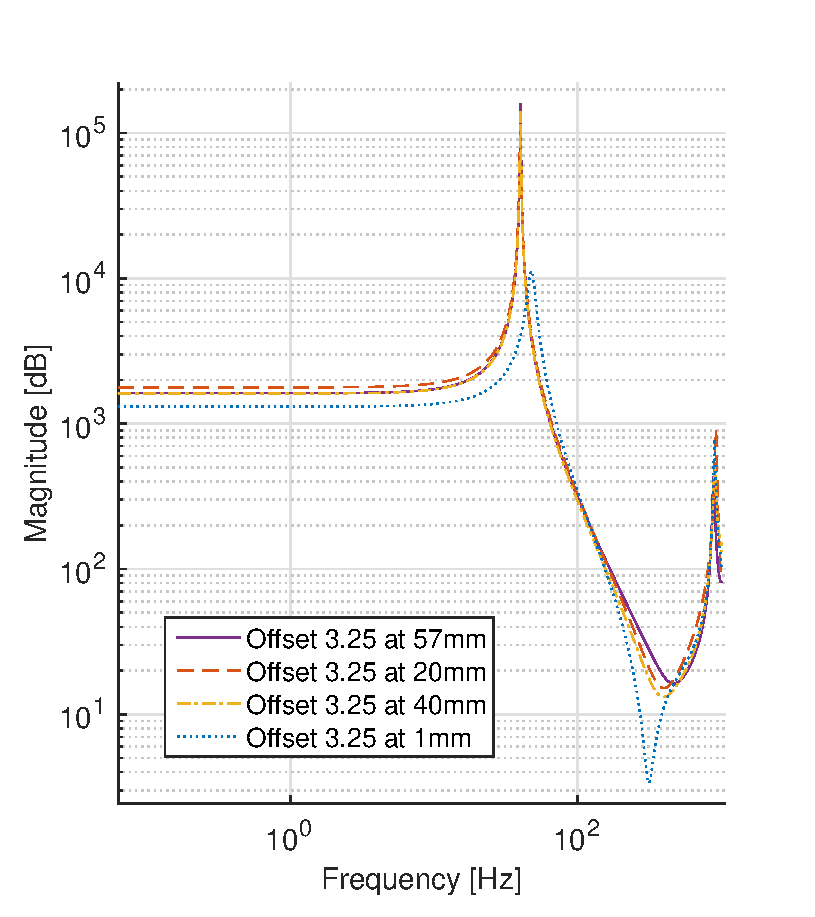
\includegraphics[width=0.4\textwidth, trim=0cm 0cm 0.8cm 1cm, clip=true]{../fig/matlab/modelcomparison2.eps}}
    \caption{\label{fig:different_lin_angle} Identified models with different rotational positions (linear axis in 54.24 mm) is shown in (a) and with different linear axis positions (rotational position corresponding to 3.25 V) is shown in (b).}
  \end{figure}
\end{frame}

\begin{frame}{Present Control Approach}
  2-DOF structure, feedback and prefilter.
  C is a series combination of a:
  \begin{itemize}
    \item  \alert{PID} - for stablity
    \item  \alert{Notch filter} - to cancel high frequency oscillations
    \item  \alert{Lead filter} - to increase the phase margin
  \end{itemize}

  \begin{figure}[h!]
    \centering %crop: left bottom right top
    \includegraphics[width=0.95\textwidth, trim=4cm 4cm 2.1cm 10cm, clip=true]{../fig/matlab/present_controller}
    \caption{\label{fig:present}Block diagram of the present control loop, including controller, prefilter and hysteresis compensator.}
  \end{figure}
\end{frame}

\section{Approaches and Simulation Results}

\begin{frame}{Model Reference Adaptive Controller}
  \alert{Idea}: Adapt to model changes and compensate for nonlinear effects.
  \begin{itemize}
    \item Uses a reference model to create the desired system response.
    \item Based on Lyapunov theory
    \item Sufficient with a low order model
    \item Nonlinear effects is seen as lumped perturbations.

  \end{itemize}
\end{frame}

\begin{frame}{Model Reference Adaptive Controller}
  System model
    \begin{equation*}
      \label{eq:sysmodel}
      \ddot{x}(t) + \alpha_1\dot{x}(t) +  \alpha_0x(t) = \beta_0u(t) + f(t)
    \end{equation*}
  Reference model
    \begin{equation*}
      \label{eq:refmodel}
      \ddot{x}_m(t) + a_1\dot{x}_m(t) +  a_0x_m(t) = b_0u_d(t)
    \end{equation*}
  Final control law
    \begin{equation*}
        \label{eq:adaplawsfinal}
      u(t) = k_0u_d(t) + (k_1 + k_3\alpha_0)x(t) +  (k_2 + k_3\alpha_1)\dot{x}(t) + k_3\ddot{x}(t) - k_3\beta_0u(t-T_s)
    \end{equation*}
    where the control law parameters are calculated as outlined below.
    \begin{equation*}
      \label{eq:adaplaws1}
      \dot{k}_0 = -\eta_0\hat{e}u_d
    \end{equation*}
    \begin{equation*}
      \label{eq:adaplaws2}
      \dot{k}_1 = -\eta_1\hat{e}x
    \end{equation*}
    \begin{equation*}
      \label{eq:adaplaws3}
      \dot{k}_2 = -\eta_2\hat{e}\dot{x}
    \end{equation*}
    \begin{equation*}
      \label{eq:adaplaws4}
      \dot{k}_3 = -\eta_3\hat{e}\hat{f}
    \end{equation*}
\end{frame}

\begin{frame}{Model Reference Adaptive Controller}
  \begin{figure}[h]
    \centering %crop: left bottom right top
    \includegraphics[width=0.75\textwidth, trim=5cm 0cm 3.8cm 0cm, clip=true]{../fig/matlab/adaptive_scheme}
    \caption{\label{fig:adaptive}Block diagram of the adaptive controller}
  \end{figure}
\end{frame}

\begin{frame}{Model Reference Adaptive Controller}
  Periodic response with model parameter drift increased linearly from $t=$ 5 s to $t=$ 7 s.
  \begin{figure}[h!]
    \centering %crop: left bottom right top
    \subfloat[][\label{fig:modelerrorresponse}Periodic response]{
    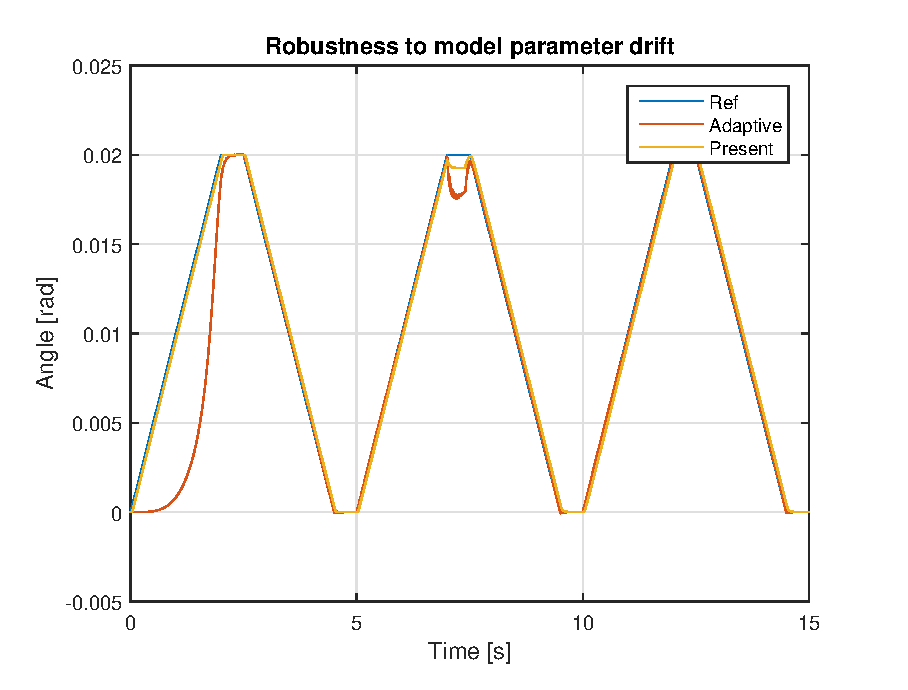
\includegraphics[width=0.4\textwidth, trim=0cm 0cm 1cm 0cm, clip=true]{../fig/matlab/modelerrorperiodic.eps}}
    \qquad
    \subfloat[][\label{fig:modelerrorbode}Model change]{
    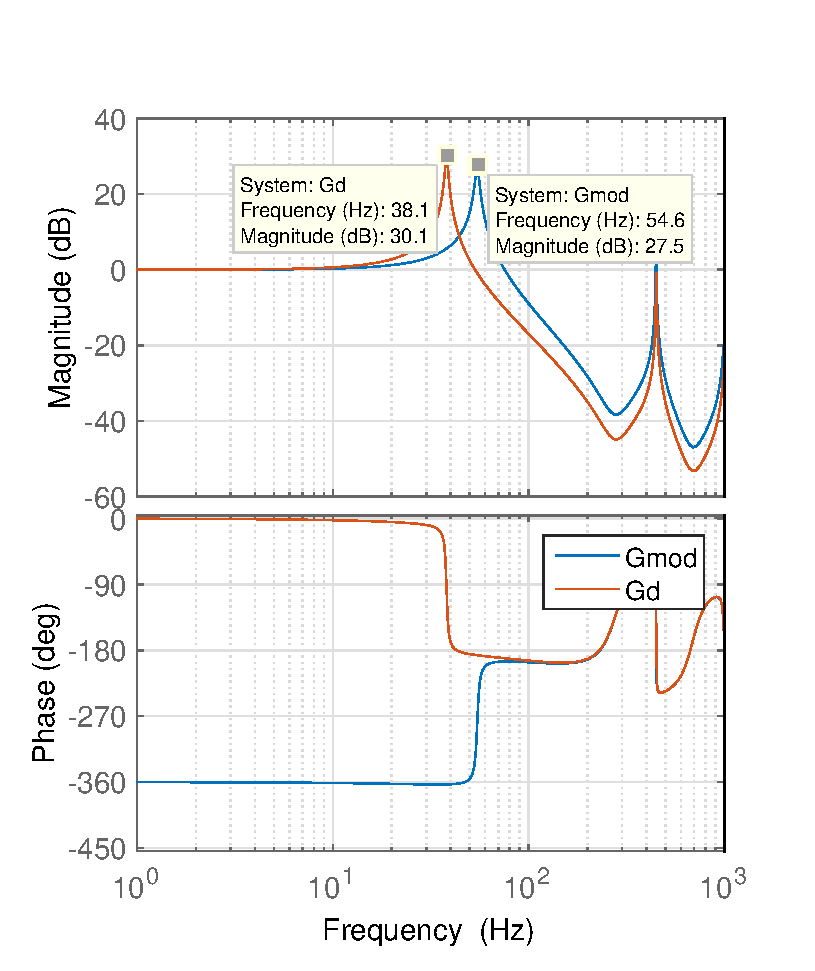
\includegraphics[width=0.42\textwidth, trim=0cm 0cm 0.7cm 0cm, clip=true]{../fig/matlab/bode_modelerror_pole.eps}}
  \end{figure}
\end{frame}

\begin{frame}{Model Reference Adaptive Controller}
  Periodic response with model parameter drift increased linearly from $t=$ 7 s to $t=$ 9 s.
  \begin{figure}[h!]
    \centering %crop: left bottom right top
    \subfloat[][\label{fig:modeldriftresponse}Periodic response]{
    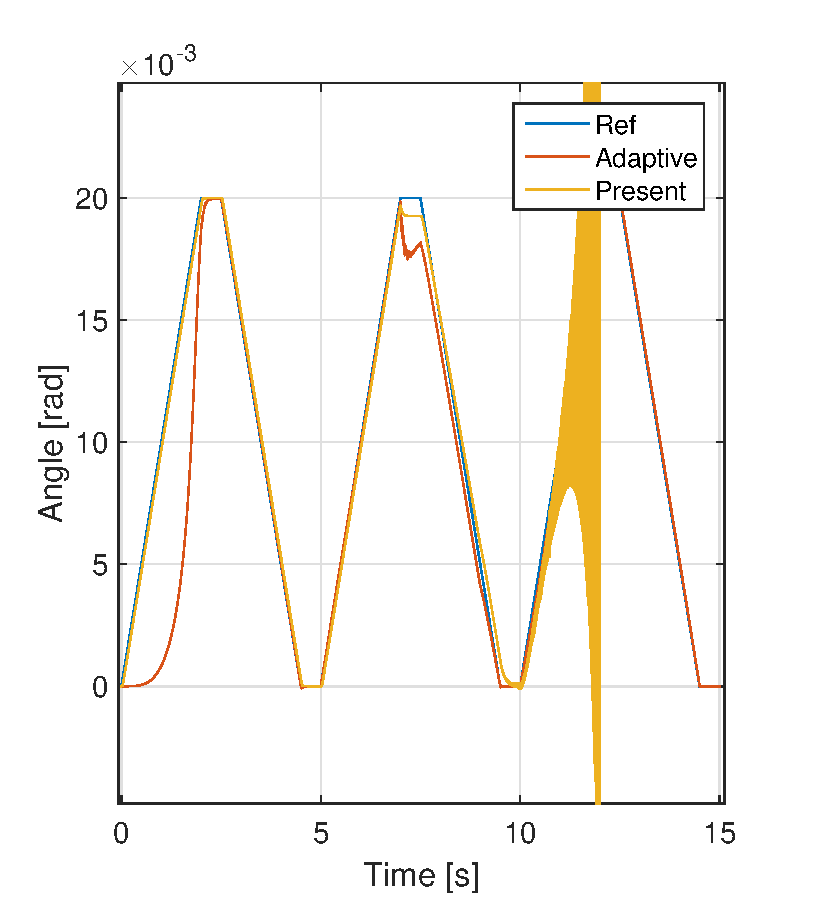
\includegraphics[width=0.4\textwidth, trim=0cm 0cm 1cm 0cm, clip=true]{../fig/matlab/driftofmodelparameterover2s.eps}}
    \qquad
    \subfloat[][\label{fig:modeldriftbode}Model change]{
    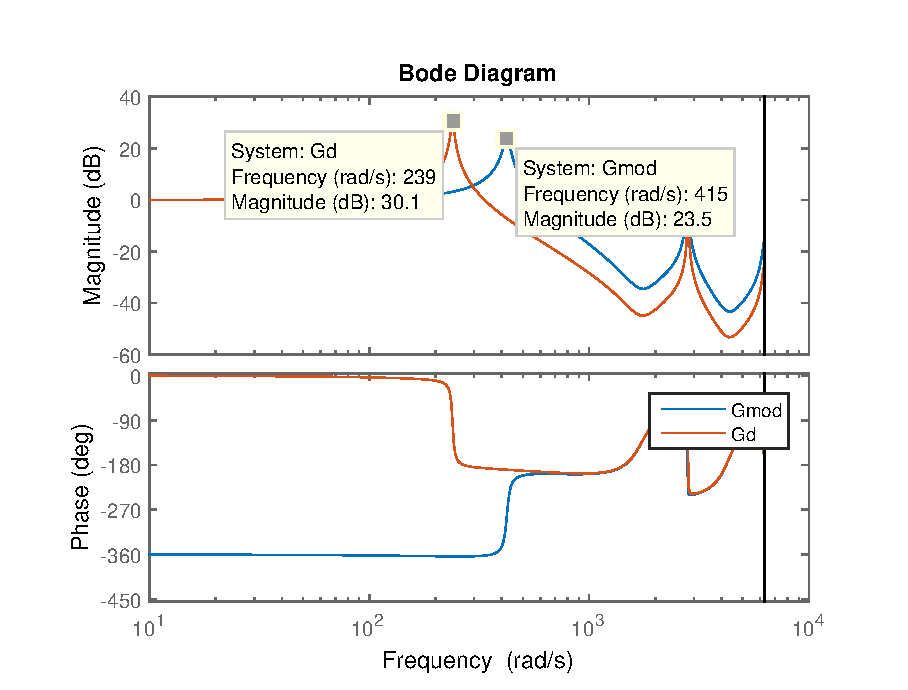
\includegraphics[width=0.42\textwidth, trim=0cm 0cm 0.7cm 0cm, clip=true]{../fig/matlab/bode_drift_pole.eps}}
  \end{figure}
\end{frame}

\begin{frame}{Model Reference Adaptive Controller}
  Tracking error
  \begin{figure}[h!]
    \centering
    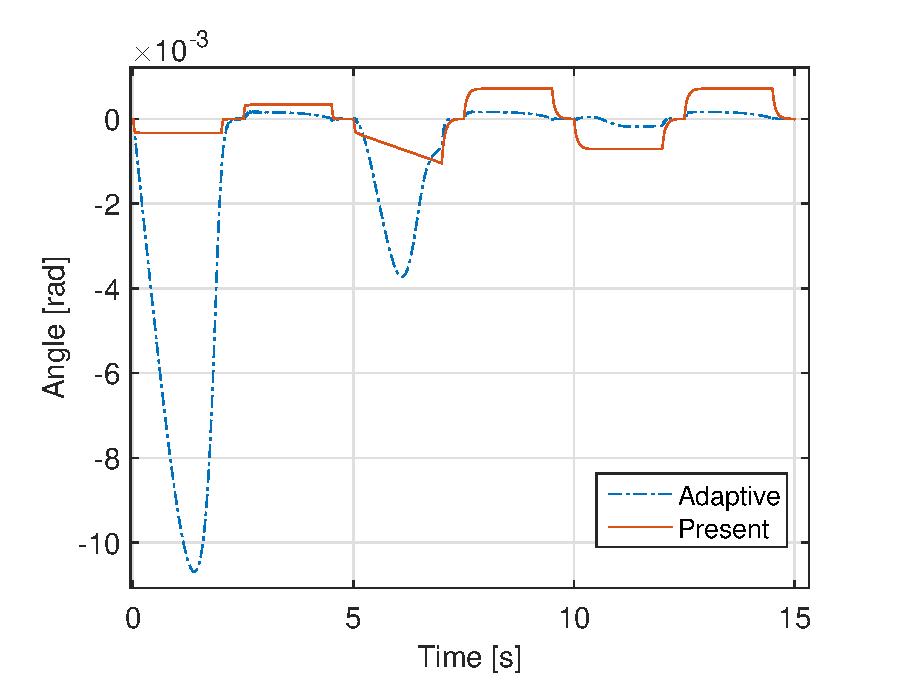
\includegraphics[width=0.7\textwidth]{../fig/matlab/modelerrorperiodic_trackingerror.eps}
    %\caption{\label{fig:modelerror_trackingerror} Tracking error of the periodic response with model errors increased linearly from $t=$ 5 s to $t=$ 7 s shown in Figure~\ref{fig:modelerror}.}
  \end{figure}
\end{frame}

\begin{frame}{Model Reference Adaptive Controller}
  \begin{figure}[h!]
    \centering %crop: left bottom right top
    \subfloat[][\label{fig:distmeas}Step response]{
    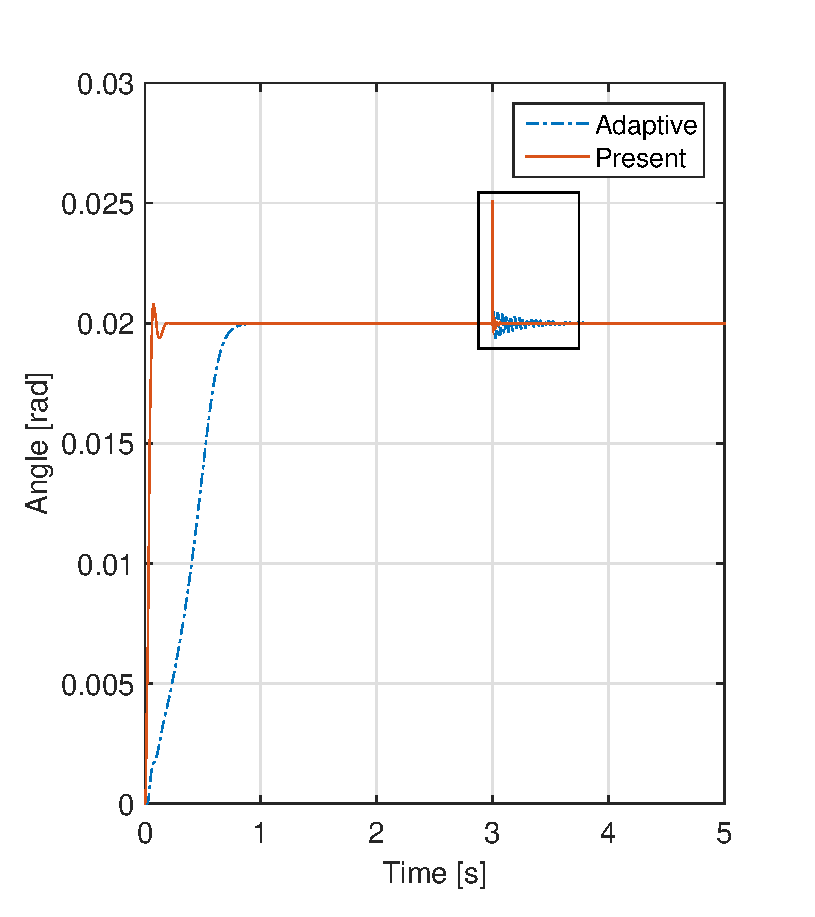
\includegraphics[width=0.43\textwidth, trim=0cm 0cm 1cm 0.8cm, clip=true]{../fig/matlab/distrejection_meas.eps}}
    \qquad
    \subfloat[][\label{fig:distmeaszoom}Zoom-in on disturbance]{
    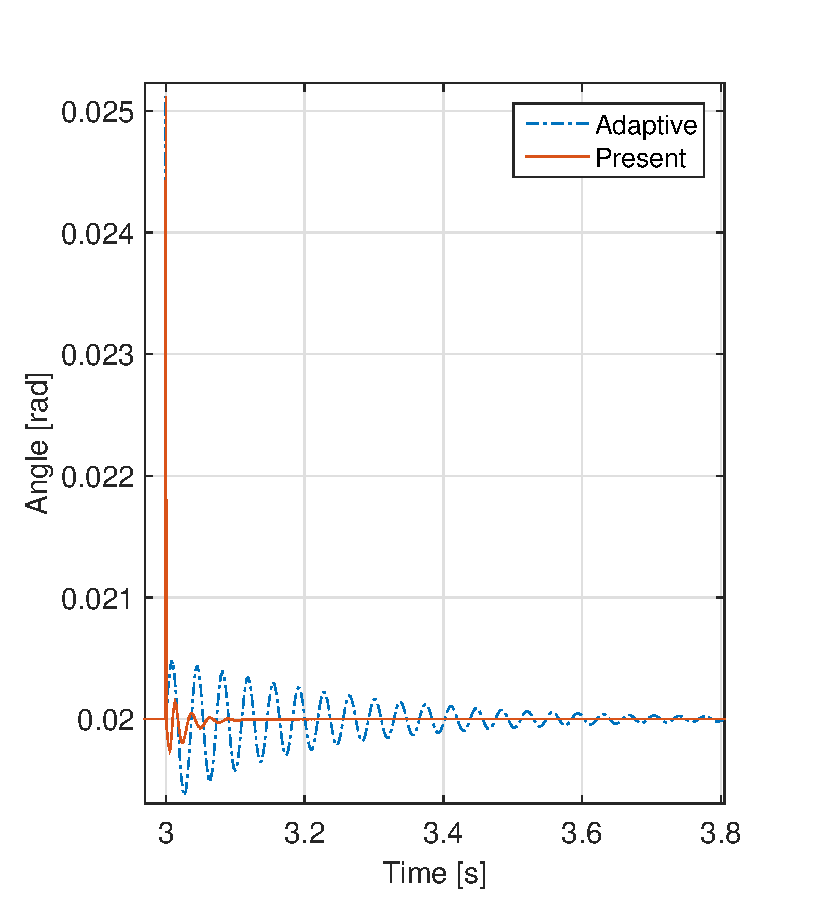
\includegraphics[width=0.43\textwidth, trim=0cm 0cm 1cm 0.8cm, clip=true]{../fig/matlab/distrejection_meas_zoom.eps}}
    %\caption{\label{fig:distmeasrejection} Step response with a disturbance impulse (amplitude of 5.1 mrad) added to the output of the system at $t=$ 3 s. The whole step response is shown in (a) with a zoom-in on the disturbance in (b).}
  \end{figure}
\end{frame}

\begin{frame}{Integral Resonance Control}
  \alert{Idea}: Increase the tracking accuracy and reduce the sensitiveness to model errors.
  \begin{itemize}
    \item Uses a constant feed-through term to damp out the first resonance peak
    \item Simple integral controller is used for inner-loop stability
    \item Increases the closed loop bandwidth implying in a better tracking performance.
    \item Interesting for long and short term effects.
  \end{itemize}
\end{frame}

\begin{frame}{Integral Resonance Control}
  \begin{figure}[h]
    \centering %crop: left bottom right top
    \includegraphics[width=0.85\textwidth, trim=5.5cm 4cm 5.1cm 9.5cm, clip=true]{../fig/matlab/irc}
    \caption{\label{fig:irc}Block diagram of the IRC damping loop.}
  \end{figure}
  \begin{equation}
    \label{eq:C2}
    C_2(s) = \frac{C(s)}{1+C(s)D_f}\Bigg|_{C(s) = \frac{-k}{s}} = \frac{-k}{s - kD_f}
  \end{equation}
\end{frame}

\begin{frame}{Integral Resonance Control}
  \begin{figure}[h]
    \centering %crop: left bottom right top
    \includegraphics[width=0.95\textwidth, trim=4cm 5cm 3.6cm 9.5cm, clip=true]{../fig/matlab/irc_int}
    \caption{\label{fig:irc_int}Block diagram of the tracking control system with IRC included.}
  \end{figure}
  \begin{subequations}
    \label{eq:discrsys}
    \begin{alignat}{2}
      & G_c(s) = \frac{C_1(s)C_2(s)G(s)}{1 + C_2(s)G(s) + C_1(s)C_2(s)G(s)} \\
      & S(s) = \frac{1}{1 + C_2(s)G(s) + C_1(s)C_2(s)G(s)} \label{eq:discrsys1}
    \end{alignat}
  \end{subequations}
\end{frame}

\begin{frame}{Integral Resonance Control}
  IRC-damping. Bode diagram of inner loop.
  \begin{figure}[h!]
    \centering
    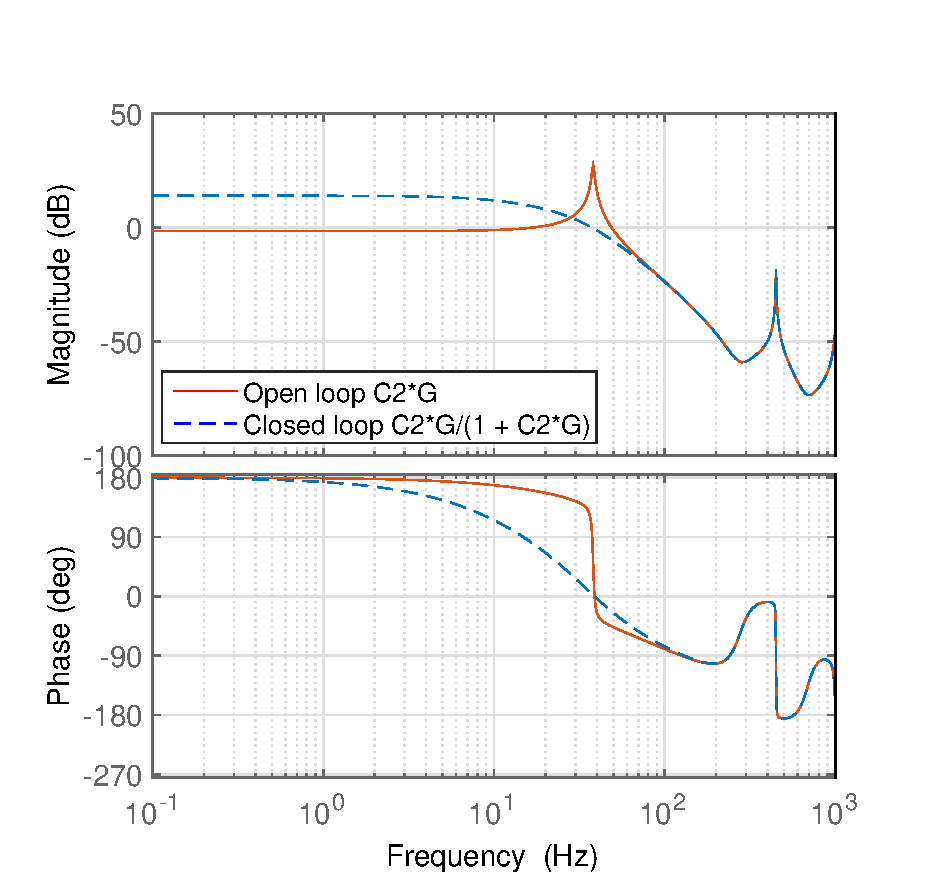
\includegraphics[width=0.7\textwidth]{../fig/matlab/bodedamped2}
    %\caption{\label{fig:bodedamped} Bode plot of the discretized open and closed loop of the \abbrIRC damping loop i.e. the inner loop of the total control loop depicted in Figure~\ref{fig:irc}.}
  \end{figure}
\end{frame}

\begin{frame}{Integral Resonance Control}
  Increased the closed loop bandwidth from 11 Hz to 73 Hz.
  \begin{figure}[h!]
    \centering
    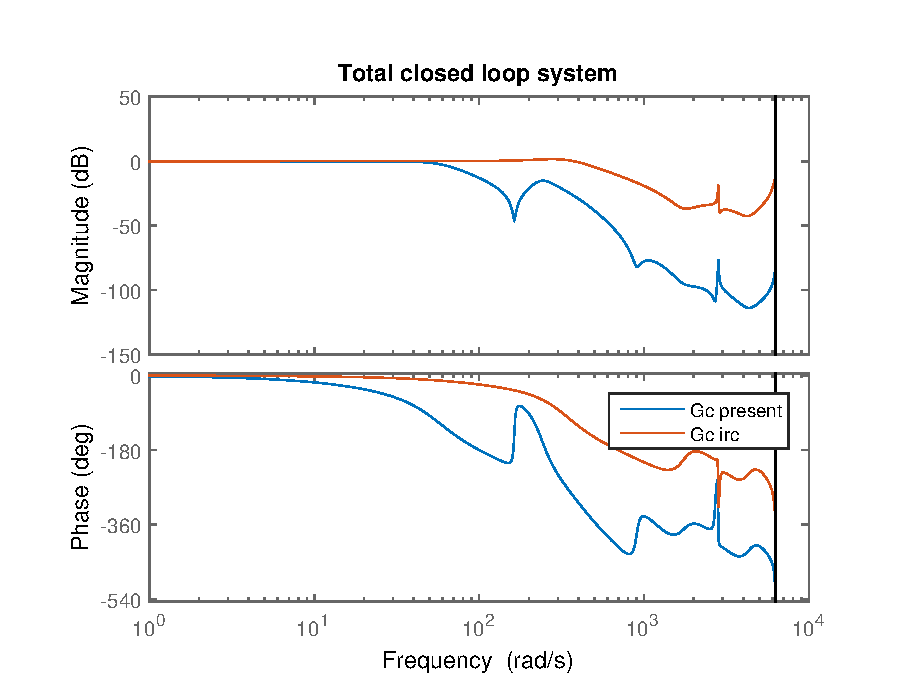
\includegraphics[width=0.7\textwidth]{../fig/matlab/totalclosedloop.eps}
    %\caption{\label{fig:irc_totalclosed} Bode plot of the discretized closed loop system of the outer control loop for the IRC depicted in Figure~\ref{fig:irc_int} and the present closed loop system.}
  \end{figure}
\end{frame}

\begin{frame}{Integral Resonance Control}
  Periodic response with model parameter drift increased linearly from $t=$ 5 s to $t=$ 7 s.
  \begin{figure}[h!]
    \centering %crop: left bottom right top
    \subfloat[][\label{fig:irc_dist_model}Periodic response]{
    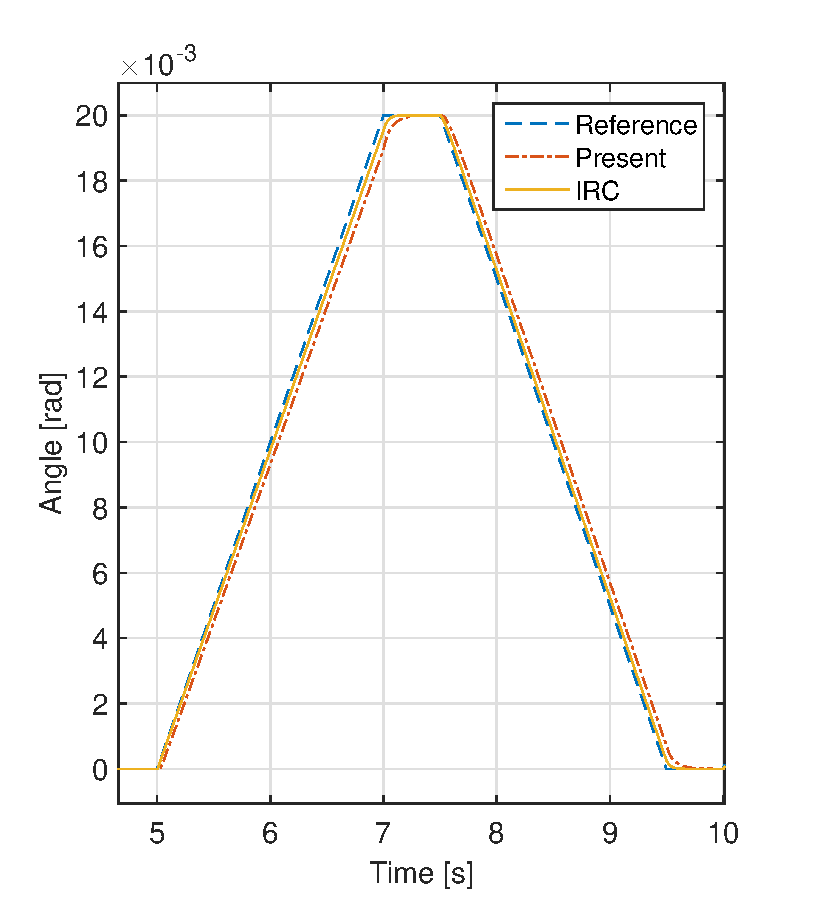
\includegraphics[width=0.43\textwidth, trim=0cm 0cm 1cm 0cm, clip=true]{../fig/matlab/irc_periodic_drift.eps}}
    \qquad
    \subfloat[][\label{fig:irc_dist_model_drift}Tracking error]{
    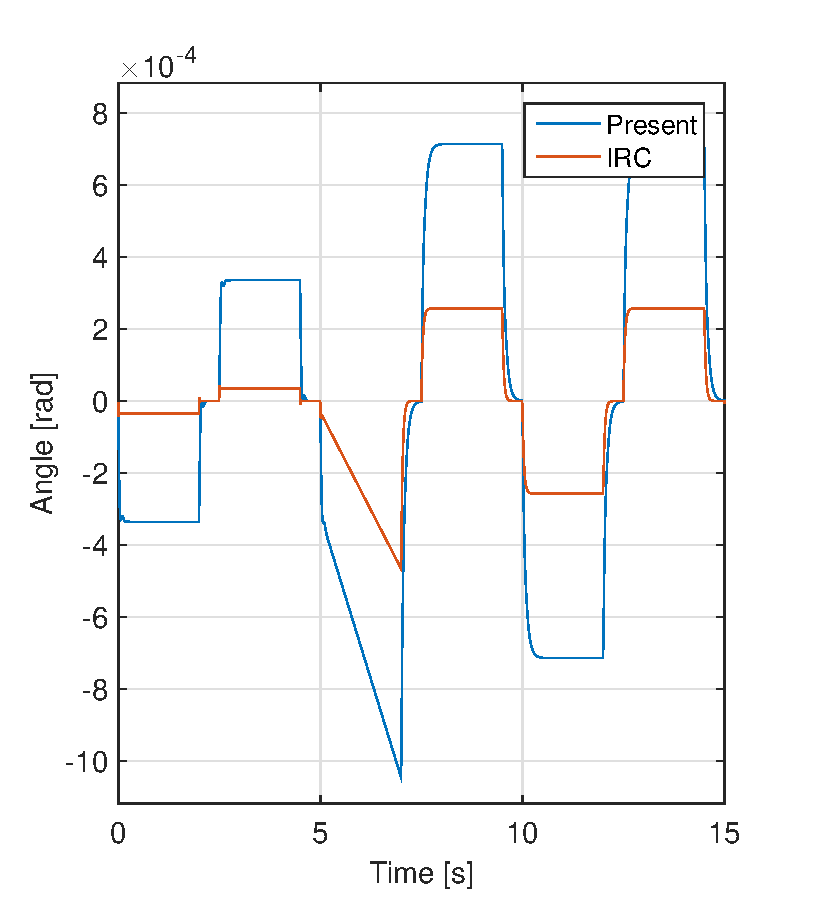
\includegraphics[width=0.43\textwidth, trim=0cm 0cm 1cm 0cm, clip=true]{../fig/matlab/irc_periodic_trackingerror.eps}}
    %\caption{\label{fig:irc_dist} Periodical input response with induced model errors for the \abbrIRC and the present controller. The model error is increased linearly from $t=$ 5 s to $t=$ 7 s. The resulting responses are shown in (a) with the tracking error is shown in (b).}
  \end{figure}
\end{frame}

\begin{frame}{Integral Resonance Control}
  \begin{figure}[h!]
    \centering
    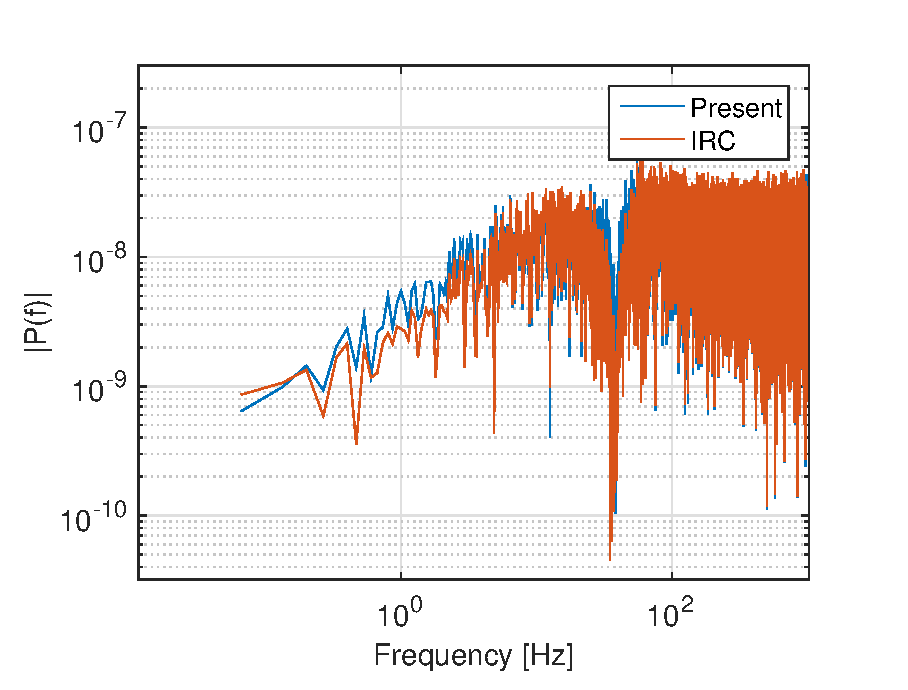
\includegraphics[width=0.7\textwidth]{../fig/matlab/whitenoiseoutput.eps}
    %\caption{\label{fig:fft_in} The \abbrFFT of the output signal from the \abbrIRC and the present closed loop system when applying white noise to the output of the system.}
  \end{figure}
\end{frame}

\begin{frame}{Harmonic Cancellation}
  \alert{Idea}: Cancel out specific disturbances coming from the environment in the tunnel or the linear stage movement.
  \begin{itemize}
    \item Feedforward Disturbance Cancellation
    \item Cancellation with Internal Model Principle
    \item Repetitive Feedforward Disturbance Cancellation
  \end{itemize}
\end{frame}

\begin{frame}{Feedforward Disturbance Cancellation}
  \alert{Idea}: Use a feedforward approach to cancel out known disturbances coming from the linear axis movement.
  \begin{itemize}
    \item Identify a static disturbance model
    \item Use the stepping signal as input to the model
    \item Disturbance must be measurable
  \end{itemize}
\end{frame}

\begin{frame}{Feedforward Disturbance Cancellation}
  \begin{figure}[h]
    \centering %crop: left bottom right top
    \includegraphics[width=0.8\textwidth, trim=8cm 4.5cm 5.97cm 8.5cm, clip=true]{../fig/matlab/ffdist}
    %\caption{\label{fig:ffdist}Block diagram of a control structure with feedforward from a known modeled disturbance.}
  \end{figure}
  \begin{equation}
    \label{eq:ffdist}
    Y(s) = \frac{C(s)G(s)}{1+C(s)G(s)}R(s) + \frac{P_d(s) - K_f(s)G(s)}{1+C(s)G(s)}D_0(s)
  \end{equation}
  Ideal choice: $K_f(s)=P_d(s)/G(s)$

   $K_f(s)$ not implementable (stable, proper and causal). $\implies$
   Approximate $G$.
\end{frame}

\begin{frame}{Feedforward Disturbance Cancellation}
  \begin{figure}[h!]
    \centering %crop: left bottom right top
    \subfloat[][\label{fig:stepin}Impulse used as input signal]{
    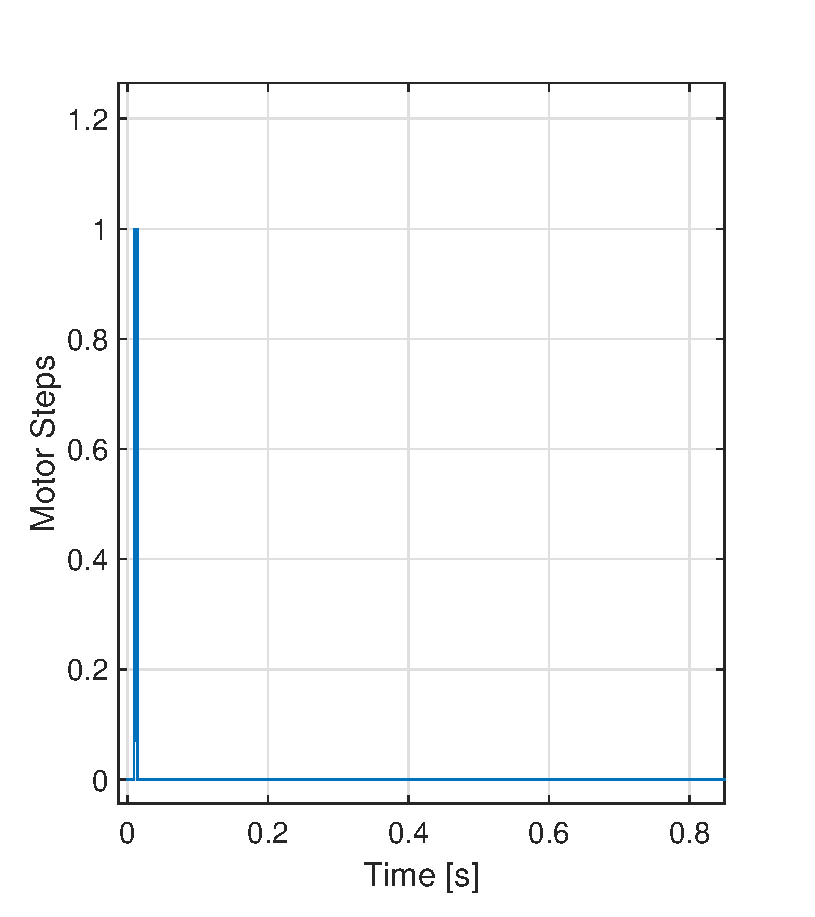
\includegraphics[width=0.43\textwidth, trim=0cm 0cm 1cm 0.8cm, clip=true]{../fig/matlab/ff_impulse.eps}}
    \qquad
    \subfloat[][\label{fig:stepout}Mean of impulse responses]{
    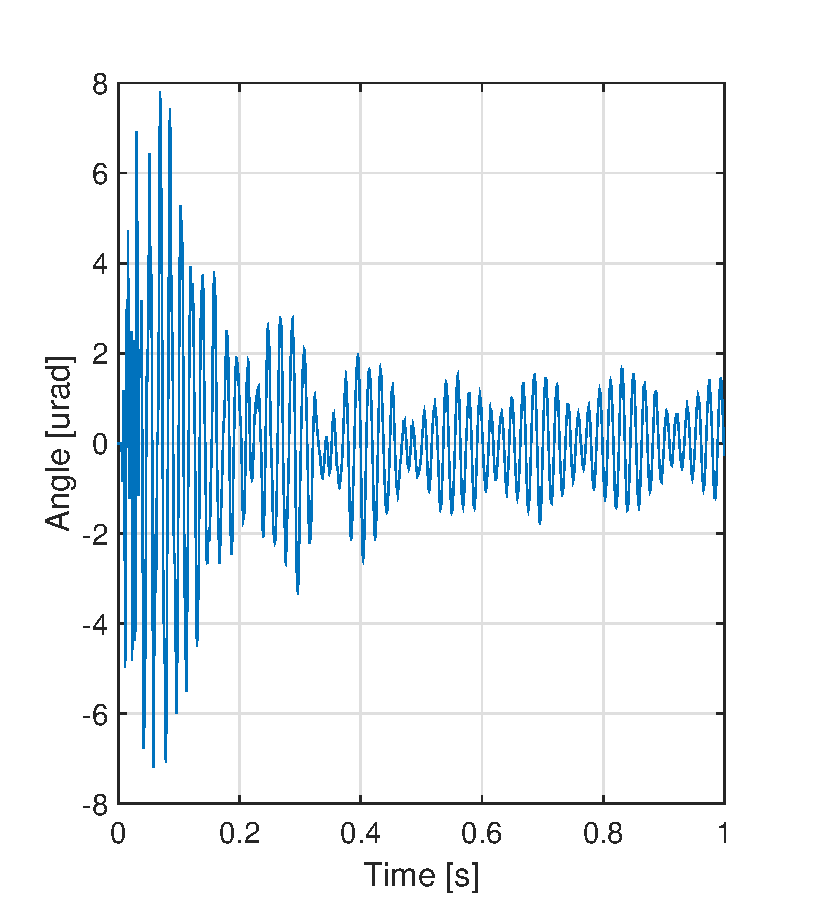
\includegraphics[ width=0.43\textwidth, trim=0cm 0cm 1cm 0.8cm, clip=true]{../fig/matlab/yaw_angle_mean_1_step_s.eps}}
    %\caption{\label{fig:stepinout} Input signal (a) and step response (b) used for modeling the disturbance. The step response was calculated by taking the mean of 50 time-synchronized acquired step responses at a movement of 1 step/s.}
  \end{figure}
\end{frame}

\begin{frame}{Feedforward Disturbance Cancellation}
  \begin{figure}[h!]
    \centering %crop: left bottom right top
    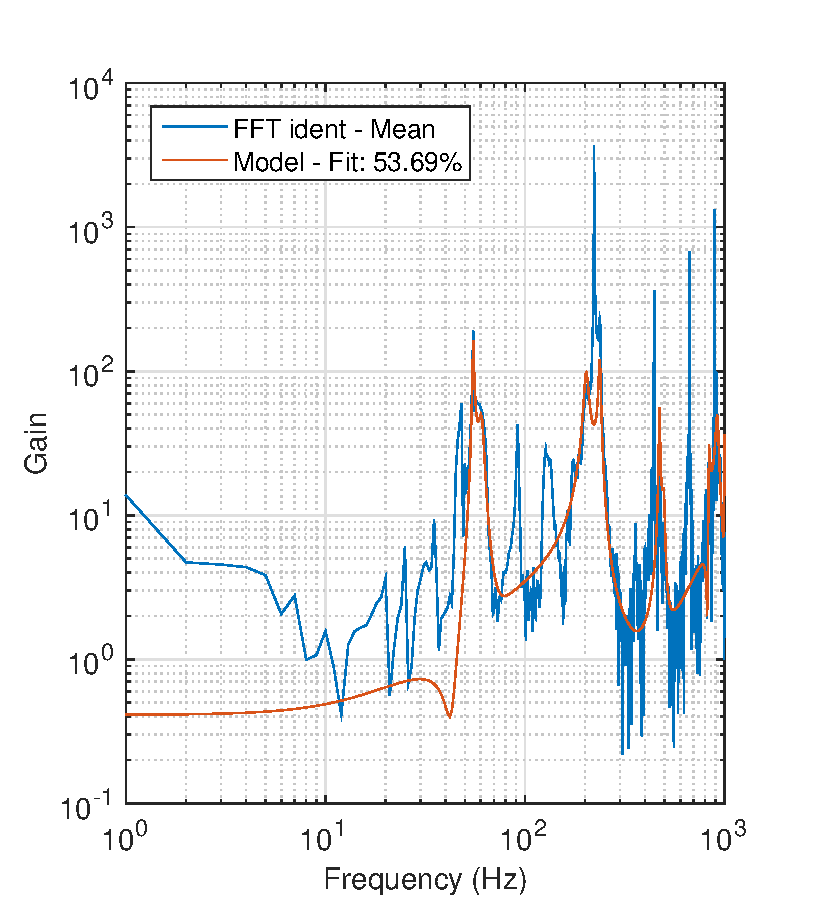
\includegraphics[width=0.6\textwidth,]{../fig/matlab/model_fit_1step_s.eps}
    %\caption{\label{fig:imp}Block diagram of the \abbrIMP control structure.}
  \end{figure}
\end{frame}

\begin{frame}{Feedforward Disturbance Cancellation}
  \begin{figure}[h!]
    \centering %crop: left bottom right top
    \subfloat[][Mean as disturbance]{
    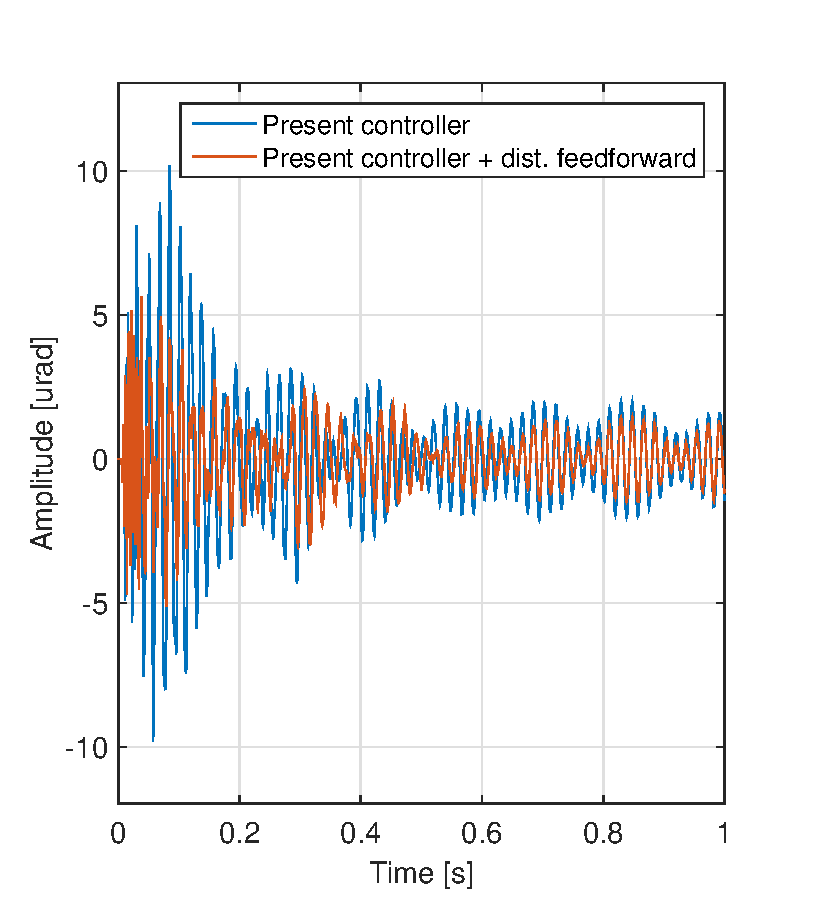
\includegraphics[width=0.43\textwidth, trim=0cm 0cm 1cm 0cm, clip=true]{../fig/matlab/cancellation_1_step_s.eps}}
    \qquad
    \subfloat[][Original acquired signal as disturbance ]{
    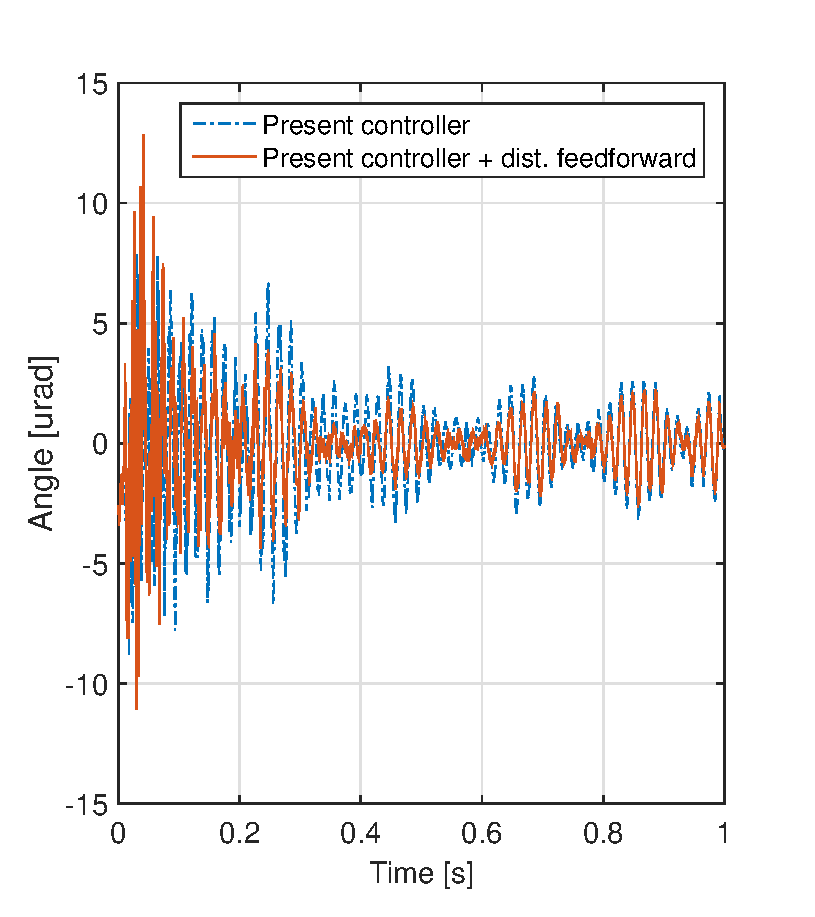
\includegraphics[width=0.43\textwidth, trim=0cm 0cm 1cm 0cm, clip=true]{../fig/matlab/cancellation_1_step_s_real_dist.eps}}
    %\caption{\label{fig:benchmark_dist} Feedforward disturbance cancellation with the mean of the acquired response added as disturbance (a) and one period of the acquired response added as disturbance (b). The disturbance cancellation is less effective with a slightly different disturbance.}
  \end{figure}
\end{frame}

\begin{frame}{Cancellation with Internal Model Principle}
  \alert{Idea}: Include a inverse model of the disturbance in the feedback loop to cancel the harmonic.
  \begin{itemize}
    \item Asymptotically reject the modeled disturbance
    \item Affecting the closed loop system
  \end{itemize}
\end{frame}

\begin{frame}{Cancellation with Internal Model Principle}
  \begin{figure}[h!]
    \centering %crop: left bottom right top
    \includegraphics[width=0.8\textwidth, trim=6.5cm 5.5cm 5.97cm 11cm, clip=true]{../fig/matlab/imp}
    %\caption{\label{fig:imp}Block diagram of the \abbrIMP control structure.}
  \end{figure}

  The generating polynomial $\Gamma(s) = f(0,s)/D(s)$.
  $C_{t}(s) = P(s)/(\Gamma(s)\bar{L}(s))$.
\end{frame}

\begin{frame}{Cancellation with Internal Model Principle}
  \begin{figure}[h!]
    \centering %crop: left bottom right top
    \subfloat[][Closed loop system]{
    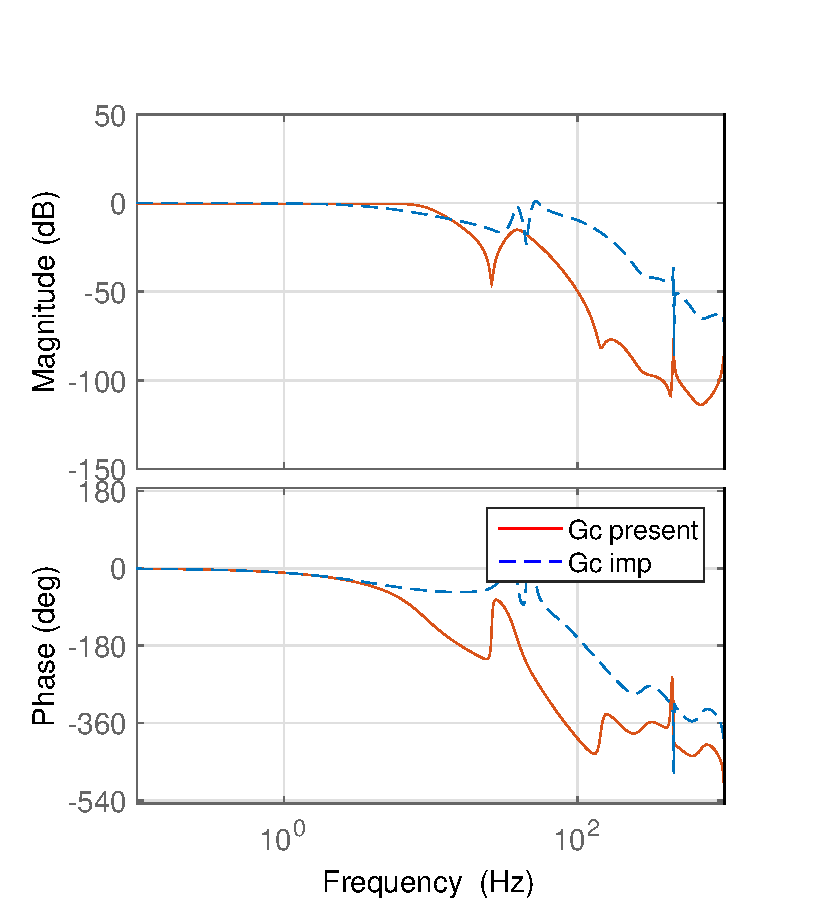
\includegraphics[width=0.43\textwidth, trim=0cm 0cm 1cm 0cm, clip=true]{../fig/matlab/gc_imp.eps}}
    \qquad
    \subfloat[][Sensitivity function]{
    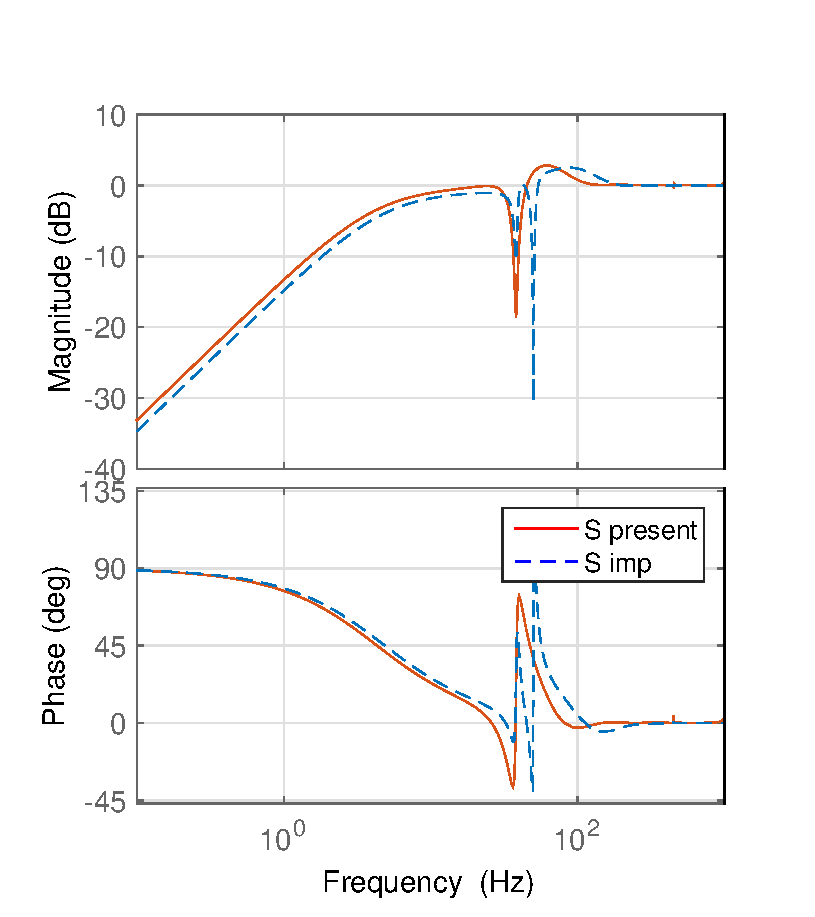
\includegraphics[width=0.43\textwidth, trim=0cm 0cm 1cm 0cm, clip=true]{../fig/matlab/s_imp.eps}}
    %\caption{\label{fig:rfdc_s_gc} Bode plot of the closed loop system shown in (a) and the sensitivity function (from output disturbance to system output) shown in (b) of the \abbrIMP and the present controller. The \abbrIMP is now attenuating disturbances at 50 Hz as seen in (b).}
  \end{figure}
\end{frame}

\begin{frame}{Cancellation with Internal Model Principle}
  \begin{figure}[h!]
    \centering %crop: left bottom right top
    \subfloat[][\label{fig:imp_model_error1}Attenuation of selected frequency]{
    \includegraphics[width=0.43\textwidth, trim=0cm 0cm 1cm 0cm, clip=true]{../fig/matlab/imp_model_error_real50.eps}}
    \qquad
    \subfloat[][\label{fig:imp_model_error2}Impact on 130 Hz component]{
    \includegraphics[width=0.43\textwidth, trim=0cm 0cm 1cm 0cm, clip=true]{../fig/matlab/imp_model_error_real.eps}}
    %\caption{\label{fig:imp_model_error}  Disturbance cancellation effectiveness with model errors. The attenuation of the major frequency is shown in (a) and the unwanted attenuation of the 130 Hz component is shown in (b).}
  \end{figure}
\end{frame}

\begin{frame}{Repetitive Feedforward Disturbance Cancellation}
  \alert{Idea}: Use an observer to estimate and cancel known disturbances without affecting the closed loop system.
  \begin{itemize}
    \item First introduced for the control of hard disks
    \item Feedforward switching mechanism with an observer
    \item Disturbance is observed, saved and replicated
    \item Reject multiple disturbances
  \end{itemize}
\end{frame}

\begin{frame}{Repetitive Feedforward Disturbance Cancellation}
The state space system and observer is given as
  \begin{subequations}
    \label{eq:sys12}
    \begin{alignat}{2}
      \label{eq:sys1}
      & \mathbf{\dot{x}}(t) = \mathbf{A_cx}(t) + \mathbf{B_c}\big(u(t) + d_o(t)\big) \\
      \label{eq:sys2}
      & y(t) = \mathbf{C_cx}(t) \\
      \label{eq:dist1}
      & \mathbf{\dot{x}}_d(t) = \mathbf{A_dx_d}(t) \\
      \label{eq:dist2}
      & d_o(t) = \mathbf{C_dx_d}(t)
    \end{alignat}
  \end{subequations}

  \begin{equation}
    \label{eq:sinm}
    \mathbf{A_d} =
      \begin{bmatrix}
         0 & 1\\[0.3em]
         -w^2 & 0
       \end{bmatrix}
       \qquad
    \mathbf{C_d} =
      \begin{bmatrix}
          1 & 0\\
      \end{bmatrix}
  \end{equation}

  \begin{equation}
    \label{eq:obs}
    \mathbf{\hat{x}}[n + 1] = \mathbf{A\hat{x}}[n] + \mathbf{B}u[n] + \mathbf{K}(\mathbf{y}[n] - \mathbf{C\hat{x}}[n])
  \end{equation}

  \begin{equation}
    \label{eq:augumented}
    \mathbf{A} =
      \begin{bmatrix}
         \mathbf{A_{zs}} & \mathbf{C_{zd}B_{zs}}\\[0.3em]
         \mathbf{0} & \mathbf{A_{zd}}\\
       \end{bmatrix}
       \qquad
    \mathbf{B} =
      \begin{bmatrix}
          \mathbf{B_{zs}}\\
          \mathbf{0}
      \end{bmatrix}
       \qquad
    \mathbf{C} =
      \begin{bmatrix}
          \mathbf{C_{zs}} & \mathbf{0}\\
      \end{bmatrix}
  \end{equation}
\end{frame}

\begin{frame}{Repetitive Feedforward Disturbance Cancellation}
  \begin{figure}[h]
    \centering %crop: left bottom right top
    \includegraphics[width=0.95\textwidth, trim=6cm 5.5cm 5.2cm 5.5cm, clip=true]{../fig/matlab/ffrep}
    %\caption{\label{fig:ffrep}Block diagram of a feedforward switching mechanism including an observer and a feedback controller.}
  \end{figure}
\end{frame}

\begin{frame}{Repetitive Feedforward Disturbance Cancellation}
  Cancellation of the 60, 90 and the 200 Hz
  \begin{figure}[h!]
    \centering %crop: left bottom right top
    \subfloat[][\label{fig:3_dist} Time domain]{
    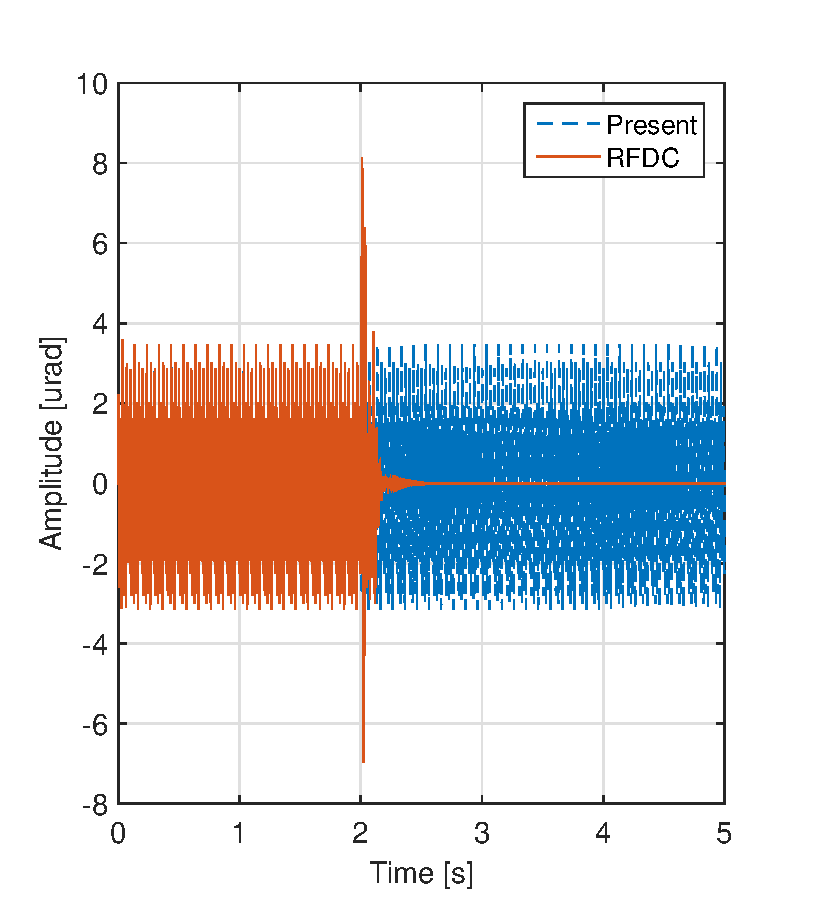
\includegraphics[width=0.43\textwidth, trim=0cm 0cm 1cm 0.8cm, clip=true]{../fig/matlab/3_dist.eps}}
    \qquad
    \subfloat[][\label{fig:3_dist_fft} FFT]{
    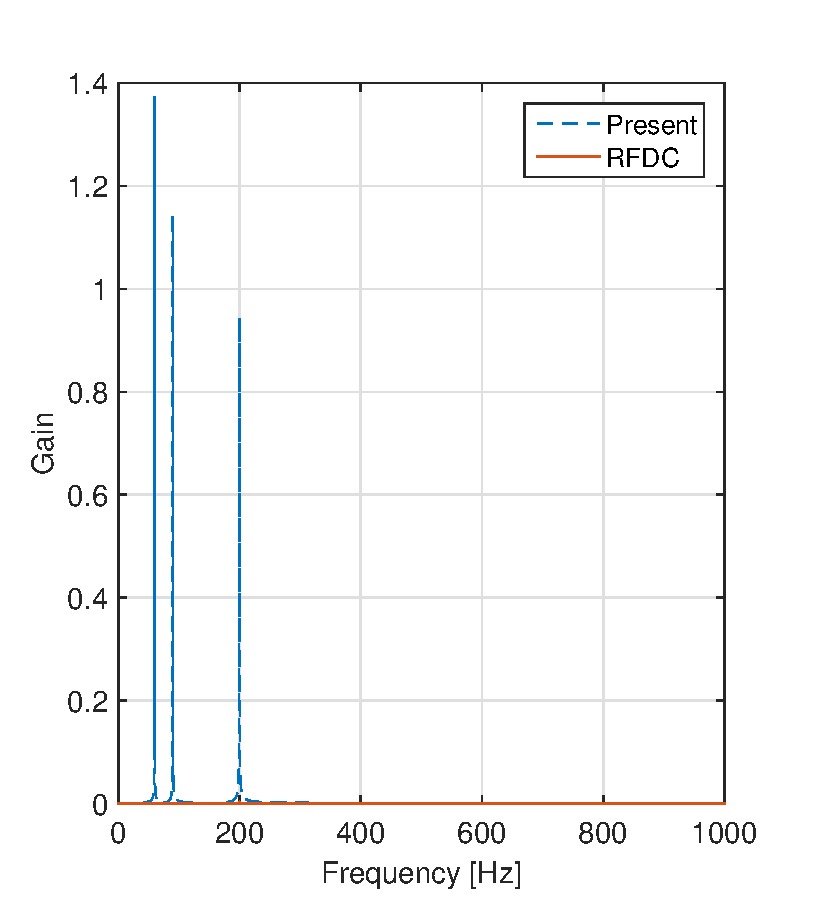
\includegraphics[width=0.43\textwidth, trim=0cm 0cm 1cm 0.8cm, clip=true]{../fig/matlab/3_dist_fft.eps}}
    %\caption{\label{fig:3_dist_both} Multiple harmonic cancellation with disturbances added to the output. The cancellation of the 60, 90 and the 200 Hz component can be seen in the time domain in (a). The \abbrFFT in (b) is performed on (a) after $t=$ 2.5 s.}
  \end{figure}
\end{frame}



\begin{frame}{Repetitive Feedforward Disturbance Cancellation}
  Multiple harmonic cancellation with real acquired disturbances
  \begin{figure}[h!]
    \centering
    \includegraphics[width=0.7\textwidth]{../fig/matlab/3real_dist_fft.eps}
    %\caption{\label{fig:fft_linear} Multiple harmonic cancellation with real acquired disturbances added to the output of the system. The figure shows the \abbrFFT with and without the \abbrRFDC active. When it is active, it attenuates the 60, 90 and the 200 Hz component efficiently. The \abbrFFT was performed after the cancellation had settled.}
  \end{figure}
\end{frame}

\begin{frame}{Repetitive Feedforward Disturbance Cancellation}
  \begin{figure}[h!]
    \centering %crop: left bottom right top
    \subfloat[][Time domain]{
    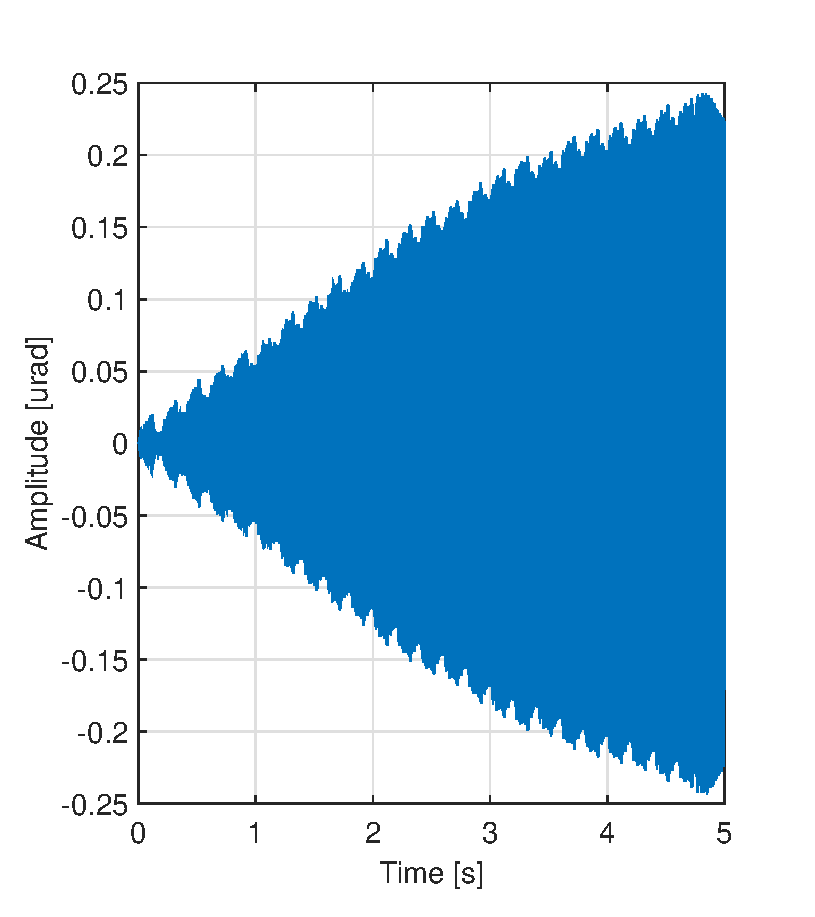
\includegraphics[width=0.43\textwidth, trim=0cm 0cm 1cm 0.8cm, clip=true]{../fig/matlab/model_conv.eps}}
    \qquad
    \subfloat[][FFT]{
    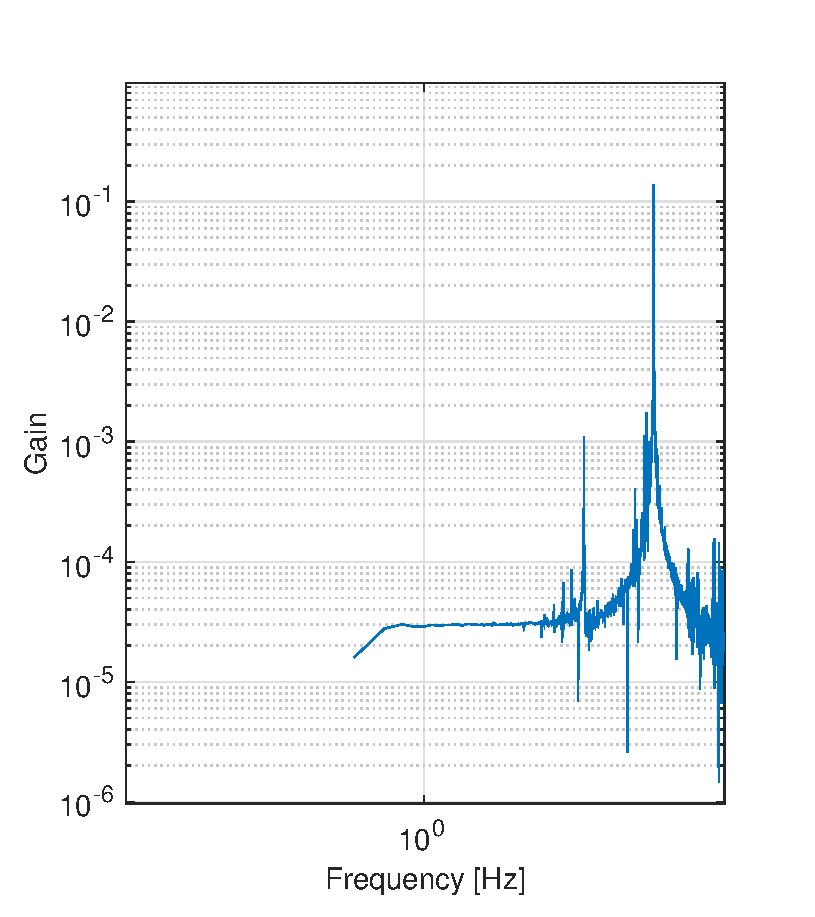
\includegraphics[width=0.43\textwidth, trim=0cm 0cm 1cm 0.8cm, clip=true]{../fig/matlab/model_conv_fft.eps}}
    %\caption{\label{fig:ph_lowgain} Observer convergence of the 200Hz harmonic with low gain, $G = [1, 0, 0, 0, 0, 0, 10, 0, 8, 0, 10, 0]^T$. The \abbrFFT of the time domain convergence (a) is presented in (b) which shows a good model of the 200 Hz harmonic.}
  \end{figure}
\end{frame}

\begin{frame}{Repetitive Feedforward Disturbance Cancellation}
  \begin{figure}[h!]
    \centering %crop: left bottom right top
    \subfloat[][Time domain]{
    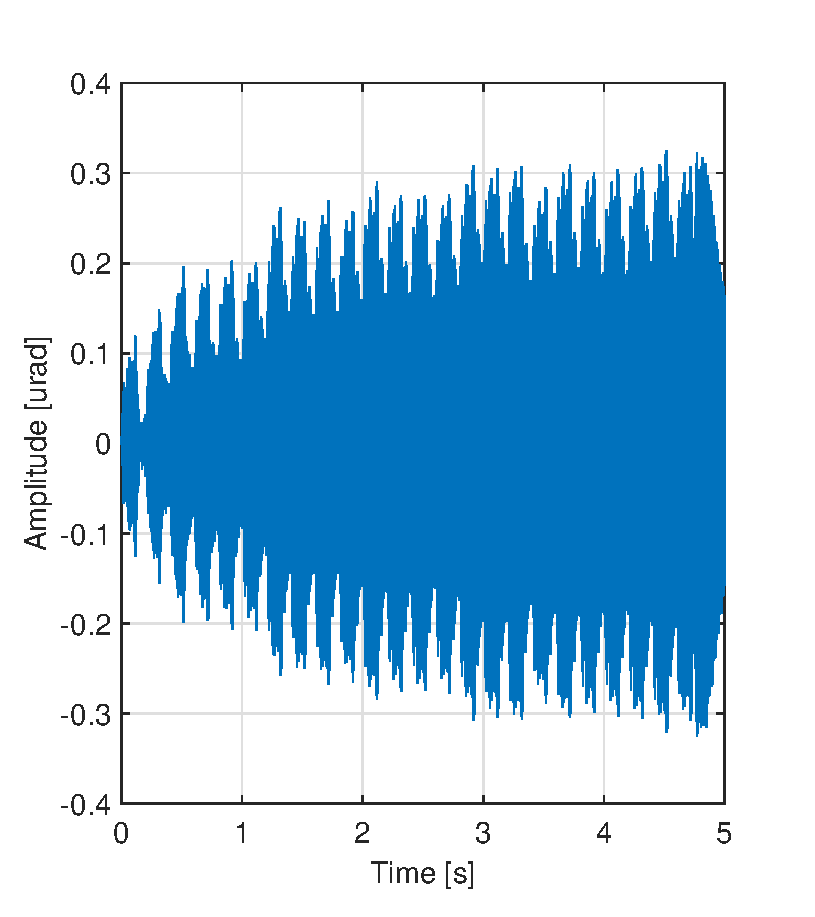
\includegraphics[width=0.43\textwidth, trim=0cm 0cm 1cm 0.8cm, clip=true]{../fig/matlab/model_conv_w.eps}}
    \qquad
    \subfloat[][FFT]{
    \includegraphics[width=0.43\textwidth, trim=0cm 0cm 1cm 0.8cm, clip=true]{../fig/matlab/model_conv_fft_w.eps}}
    %\caption{\label{fig:ph_highgain} Observer convergence of the 200Hz harmonic with high gain, $G = [1, 0, 0, 0, 0, 0, 10, 0, 8, 0, 70, 0]^T$. The \abbrFFT of the time domain convergence (a) is presented in (b) which shows a less good model of the 200 Hz harmonic with a lot of other modeled frequency components in the region of 200 Hz.}
  \end{figure}
\end{frame}

\begin{frame}{Comparison}
  \scriptsize
  \begin{table}[h!]
    \centering
    \begin{tabular}{| l | P{3cm} | P{1.8cm} | P{1.8cm} | P{1.8cm} |}
      \hline
      \bf{No} & \bf{Aspect}  & \bf{Present} & \bf{IRC} & \bf{MRACPE} \\ \hline
      1 & Closed-loop Bandwidth [Hz] & 9.7 & 73.3 & -\\ \hline
      2 & Gain/Phase margin [dB / $^{\circ}$] & 14.4/66.2 & 13.1/49.4 & -\\ \hline
      3 & Tracking error, periodic input $\sigma$-[mrads] & $0.29$ & $0.03$ & $0.11$\\ \hline
      4 & Tracking error with model errors (model's 1st resonance at 22.0Hz), $\sigma$-[mrads] & $\infty$ & 0.03 & 0.21\\ \hline
      5 & Tracking error with model errors (model's 1st resonance at 67.2Hz), $\sigma$-[mrads] & $\infty$ & 0.03 & 0.11\\ \hline
      6 & Tracking error with model errors (model's 1st resonance at 17.6Hz), $\sigma$-[mrads] & $\infty$ & $\infty$ & 0.47\\ \hline
      7 & Tracking error with model errors (model's 1st resonance at 77.7Hz), $\sigma$-[mrads] & $\infty$ & $\infty$ & 0.11\\ \hline
    \end{tabular}
    %\caption{\label{tab:comp} Key parameters for the \abbrIRC, the \abbrMRACPE and the present control approach.}
  \end{table}
\end{frame}

\begin{frame}{Comparison}
  \scriptsize
  \begin{table}[h!]
    \centering
    \begin{tabular}{| l | P{3cm} | P{1.8cm} | P{1.8cm} | P{1.8cm} |}
      \hline
      \bf{No} & \bf{Aspect}  & \bf{Present} & \bf{IRC} & \bf{MRACPE} \\ \hline
      8 & Output disturbance rejection, settling time (1\%) [ms] & 8 & 25 & 260\\ \hline
      9 & Input/Output disturbance rejection, $\sigma$-[\unit{\micro\radian}] & $0.68 $/$1.43$ & $0.45$/$1.46$ & $1.95$/$1.41$\\ \hline
      10 & Stability issues & Unstable with high model errors & Unstable with high model errors, but better than present & Good adaption even with model errors, but tuning for quicker adaption easily leads to instability.  Stability only proven in continuous time. \\ \hline
      11 & Design and implementation considerations & Straight- forward technique, allowing for basic stability analysis & Same as present & Hard to tune. High computational burden for higher order models.\\ \hline
    \end{tabular}
    %\caption{\label{tab:comp} Key parameters for the \abbrIRC, the \abbrMRACPE and the present control approach.}
  \end{table}
\end{frame}

\begin{frame}{Comparison}
  \scriptsize
  \begin{table}[h!]
    \centering
    \begin{tabular}{| l | P{3cm} | P{1.8cm} | P{1.8cm} | P{1.8cm} |}
      \hline
        \bf{No} & \bf{Aspect} & \bf{FDC} & \bf{RFDC} & \bf{IMP} \\ \hline
      1 & Affecting closed loop system & No & No & Yes\\ \hline
      2 & Cancellation effectiveness of major frequency, attenuation-[\%]                & 64.6 & 88.4 & 83.3\\ \hline
      3 & Cancellation with model errors (model's 1st resonance at 28.2Hz), attenuation-[\%] & 40.5 & 26.6 & 73.5\\ \hline
      4 & Cancellation with model errors (model's 1st resonance at 43.4Hz), attenuation-[\%] & 57.7 & 5.0 & 83.4\\ \hline
      5 & Implementation considerations & Requires high order model, computational demanding. & Requires observer, computational demanding. Can be used as add-on.& Controller must be retuned when selecting a new frequency. \\ \hline
    \end{tabular}
    %\caption{\label{tab:comp_h} Key parameters for the harmonic cancellation methodologies.}
  \end{table}
\end{frame}

\section{Implementation}

\begin{frame}{Setup}
  \begin{figure}[h]
   \centering %crop: left bottom right top
   \subfloat[][Setup]{
   \includegraphics[width=0.43\textwidth]{../fig/setup}}
   \qquad
   \subfloat[][Shaker]{
   \includegraphics[width=0.43\textwidth]{../fig/shaker}}
   %\caption{\label{fig:beateffect} Cancellation performance in closed loop of the 50 Hz component suffering from the beat effect. The standard deviation, calculated as an average of the standard deviation of (a) every 5 s, is shown in (b).}
  \end{figure}
\end{frame}

\begin{frame}{Labview Implementation}
  \begin{figure}[h]
    \centering %crop: left bottom right top
    \includegraphics[width=0.8\textwidth]{../fig/HC_gui}
    \caption{\label{fig:gui}Graphical user interface of the RFDC implementation.}
  \end{figure}
\end{frame}

\begin{frame}{Single Disturbance}
  RFDC cancellation verification with disturbance added by shaker.
  80 Hz component is reduced by 76\% of its original amplitude.
  \begin{figure}[h!]
    \centering %crop: left bottom right top
    \includegraphics[width=0.85\textwidth]{../fig/matlab/fft_closedloop_ext_disturbance_80Hz_with_zoom_2}
    %\caption{\label{fig:fft_closedloop_80} \abbrFFT of the yaw angle response acquired in closed loop with and without the \abbrRFDC active. Cancellation of the 80 Hz component generated by the shaker.}
  \end{figure}
\end{frame}

\begin{frame}{Single Disturbance}
  ... which reduces the standard deviation significantly.
  \begin{figure}[h!]
    \centering %crop: left bottom right top
    \includegraphics[width=0.8\textwidth, trim=0cm 0cm 0cm 0.7cm, clip=true]{../fig/matlab/yl_closedloop_ext_disturbance_80Hz_2}
    %\caption{\label{fig:yl_closedloop_80} Closed loop response showing the development of the yaw angle over time, with and without the \abbrRFDC active. Cancellation of the 80 Hz component generated by the shaker.}
  \end{figure}
\end{frame}

\begin{frame}{Multiple Disturbances}
  The cancellation of 50Hz and 80 Hz component under the first 10 s.
  \begin{itemize}
    \item 50Hz component reduced by 75\%
    \item  80Hz component reduced by 66\%
  \end{itemize}

  \begin{figure}[h]
    \centering %crop: left bottom right top
    \includegraphics[width=0.85\textwidth]{../fig/matlab/mult_50_80_closed_loop}
    %\caption{\label{fig:mult5080} Multiple cancellation in closed loop of the 50 and the 80 Hz component. The plot is based on a 10 s long acquisition.}
  \end{figure}
\end{frame}

\begin{frame}{Beat effect}
   Cancellation performance in closed loop over 2 minutes.
  \begin{figure}[h!]
    \centering %crop: left bottom right top
    \subfloat[][Yaw angle displacement]{
    \includegraphics[width=0.43\textwidth]{../fig/matlab/beat_effect_yl}}
    \qquad
    \subfloat[][Standard deviation]{
    \includegraphics[width=0.43\textwidth]{../fig/matlab/beat_effect}}
    %\caption{\label{fig:beateffect} Cancellation performance in closed loop of the 50 Hz component suffering from the beat effect. The standard deviation, calculated as an average of the standard deviation of (a) every 5 s, is shown in (b).}
  \end{figure}
\end{frame}

\begin{frame}{Beat effect}
  Cancellation of artificial disturbances
  \begin{figure}[h!]
    \centering %crop: left bottom right top
    \subfloat[][Yaw angle displacement]{
    \includegraphics[width=0.43\textwidth]{../fig/matlab/no_beat_effect_yl}}
    \qquad
    \subfloat[][Standard deviation]{
    \includegraphics[width=0.43\textwidth]{../fig/matlab/no_beat_effect}}
    %\caption{\label{fig:nobeat}Cancellation of artificial disturbances in open loop not suffering from beat effect. The yaw angle is shown in (a) with the standard deviation in (b). The change in the data without \abbrRFDC is due to environmental changes.}
  \end{figure}
\end{frame}

\section{Conclusion}

\begin{frame}{Simulation}
  IRC
  \begin{itemize}
    \item  Can be used to efficiently increase the closed loop bandwidth
    \item  80Hz component reduced by 66\%
  \end{itemize}
  MRACPE
  \begin{itemize}
    \item Can be used to adapt to large model changes and thereby prevent instability (way too significant)
    \item Stability depending on the step size
    \item Better for long term parameter adaption
  \end{itemize}
  RFDC
  \begin{itemize}
    \item Can be used to efficiently damp out known harmonic oscillations
    \item 80Hz component reduced by 66\%
  \end{itemize}
\end{frame}

\begin{frame}{Implementation}

\end{frame}

\begin{frame}{Summary}

\end{frame}

\begin{frame}[standout]
  Questions?
\end{frame}

\appendix

\begin{frame}[allowframebreaks]{References}

  \bibliography{pres}
  \bibliographystyle{abbrv}

\end{frame}

\end{document}
